\documentclass[table,professionalfonts]{beamer}
\usepackage{xcolor}
\usepackage{booktabs}
\usepackage{graphicx}
\usepackage{tikz}
\usepackage{feynmp}
\ifpdf
\usepackage[pdftex]{thumbpdf}
\else
\usepackage[dvips]{thumbpdf}
\fi
\usepackage[utf8]{inputenc}
\usepackage[T1]{fontenc}
%\usepackage{lmodern}
\usepackage{bbm}
%\usepackage{arev}
\usepackage{bera}
%\usepackage[light]{kpfonts}
%\usepackage[scale=.9]{tgheros}
\usepackage[scaled=1.125]{libertine}
%\usepackage{txfonts}
%\usepackage{pxfonts}
%\usepackage{utopia}
%\usepackage{charter}
%\usepackage{concrete}
%\usepackage{iwona}
%\usepackage{fourier}
%\usepackage{pandora}
%\usepackage[lf]{MinionPro}
%\usepackage{MnSymbol}
%\renewcommand{\sfdefault}{Myriad-LF}
%\usepackage[lf]{Myriad}
%\renewcommand{\rmdefault}{pnr}
%\renewcommand{\sfdefault}{pnss}
%\renewcommand{\ttdefault}{pntt}
\renewcommand{\ttdefault}{fvm}
%\usepackage{eulervm}
\ifpdf
\usepackage{epstopdf}
\usepackage[protrusion=true,expansion=true,tracking]{microtype}
%\DeclareGraphicsRule{*}{mps}{*}{}
\fi

\usepackage{listings}
\lstloadlanguages{C++}
\makeatletter
\newcommand{\srcsize}{\@setfontsize{\srcsize}{4.5pt}{4.5pt}}
\makeatother
\lstset{
        language=C++,
        basicstyle=\srcsize\ttfamily\color{red},
        keywordstyle=\color{cyan},
        commentstyle=\color{blue}\textsl,
        stringstyle=\color{magenta},
        identifierstyle=\color{black},
        breaklines=true,breakautoindent=true}

%\usetheme{CambridgeUS}
\usecolortheme{beaver}
\setbeamercolor{section in toc}{fg=black,bg=white}
\setbeamercolor{alerted text}{fg=blue}
\setbeamercolor{structure}{fg=blue!80!black}
\setbeamercolor*{palette primary}{fg=black,bg=gray!30!white}
\setbeamercolor*{palette secondary}{fg=black,bg=gray!15!white}
\setbeamercolor*{palette tertiary}{bg=blue!80!black,fg=gray!10!white}
\setbeamercolor*{palette quaternary}{fg=blue,bg=gray!5!white}
\setbeamercolor*{sidebar}{fg=blue,bg=gray!15!white}
\setbeamercolor*{palette sidebar primary}{fg=blue!10!black}
\setbeamercolor*{palette sidebar secondary}{fg=white}
\setbeamercolor*{palette sidebar tertiary}{fg=blue!50!black}
\setbeamercolor*{palette sidebar quaternary}{fg=gray!10!white}
\setbeamercolor{titlelike}{parent=palette primary,fg=blue,bg=white}
\setbeamercolor{frametitle}{fg=white,bg=blue!80!black}
\setbeamercolor{frametitle right}{bg=gray!60!white}
\setbeamercolor*{separation line}{}
\setbeamercolor*{fine separation line}{}
\useinnertheme{rectangles}
\useoutertheme{infolines}
%\usefonttheme[onlymath]{serif}
%\usefonttheme{professionalfonts}

%\loadgraphics{logo-pi-bunt3,lhcb-logo,unisiegel-gray}

\newsavebox{\unilogo} \newsavebox{\pilogo} \newsavebox{\lhcblogo}
\sbox{\unilogo}{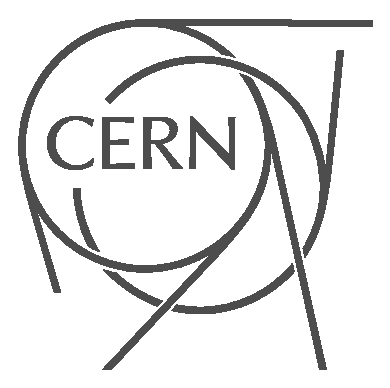
\includegraphics[height=1.2cm]{cern-logo-gray.eps}}
\sbox{\pilogo}{\includegraphics[height=0.75cm]{cern-logo.eps}}
\sbox{\lhcblogo}{
\includegraphics[height=0.75cm]{lhcb-logo.eps}}

\setbeamertemplate{footline}
{
  \leavevmode%
  \hbox{%
  \begin{beamercolorbox}[wd=.333333\paperwidth,ht=2.25ex,dp=1ex,left]{author in head/foot}%
    \usebeamerfont{author in head/foot}\vtop{\vskip-2.25ex\hbox{\resizebox{!}{3.25ex}{\usebox{\pilogo}}}}%
    \hfill \insertshortauthor~~(\insertshortinstitute) \hfill%
  \end{beamercolorbox}%
  \begin{beamercolorbox}[wd=.333333\paperwidth,ht=2.25ex,dp=1ex,center]{title in head/foot}%
    \usebeamerfont{title in head/foot}\insertshorttitle%
  \end{beamercolorbox}%
  \begin{beamercolorbox}[wd=.333333\paperwidth,ht=2.25ex,dp=1ex,right]{date in head/foot}%
    \usebeamerfont{date in head/foot}\insertshortdate{}\hspace*{2em}%
    \insertframenumber{} / \inserttotalframenumber\hspace*{2ex} \vtop{\vskip-2.25ex\hbox{\resizebox{!}{3.25ex}{\usebox{\lhcblogo}}}}%
  \end{beamercolorbox}}%
  \vskip0pt%
}

\setbeamertemplate{frametitle}
{
  \ifbeamercolorempty[bg]{frametitle}{}{\nointerlineskip}%
  \leavevmode%
  \vskip-2pt\hbox{%
  \begin{beamercolorbox}[wd=\paperwidth,left]{frametitle}%
    \usebeamerfont{frametitle}%
    \vskip.125ex%
    \hbox{\vtop{\raisebox{-1ex}[1ex][1ex]{\makebox[0pt][l]{\usebox{\unilogo}}}%
    \hspace{1em}\strut\insertframetitle\strut}\par%
    {%
      \ifx\insertframesubtitle\@empty%
      \else%
      {\usebeamerfont{framesubtitle}\usebeamercolor[fg]{framesubtitle}\insertframesubtitle\strut\par}%
      \fi
    }}%
  \end{beamercolorbox}%
  }%
}


\definecolor{bandgreen}{rgb}{0.4,0.8,0.4}
\newcommand{\FIXME}{{\color{red}FIXME}}
\newcommand{\arxiv}[1]{{\color{gray}\tiny$[$\href{http://arxiv.org/abs/#1}{arXiv:#1}$]$}}
\newcommand{\jref}[2]{{\color{gray}\tiny$[$\href{#2}{#1}$]$}}

\author[M. Schiller]{Manuel Schiller}
\institute{CERN}
\date{July 9th-10th, 2015}
\title{overview of the B2DXFitters package}

\begin{document}
\begin{fmffile}{talk-fmf}
\section[1st B2DXFitters workshop]{$\,$}
\subsection{Padova}
\maketitle

\section{introduction}
\begin{frame}{introduction}
\begin{itemize}
\item B2DXFitters is a rather versatile package
\begin{itemize}
\item can do sophisticated mass/PID fits to extract yields/sWeights \\
    {\color{blue} see Agnieszka's talk(s) and her part of the hands-on session}
\item also does rather complicated time fits \\
    {\color{blue} see my talk(s) and my part of the hands-on session}
\end{itemize}
\item a lot of effort has gone into making (time) fits fast
\begin{itemize}
\item very necessary with ever increasing data sets and fit complexities
\item would like to transfer lessons learned to next generation\ldots
\end{itemize}
\end{itemize}
\end{frame}

\begin{frame}{outline}
\begin{itemize}
\item package structure
\item start with overview of time fitting part (outline of topics later)
\item then hand over quickly to Agnieszka's ``mass fit news'' talk because I run
    out of time
\item we can and will come back to these slides during the hands-on session, I
    promise\ldots :)
\end{itemize}
\end{frame}

\section{package structure}
\begin{frame}{package structure}
    \vfill
    $\,$ \hfill {\Huge package structure} \hfill $\,$ \\
    \vfill
\end{frame}

\begin{frame}{package structure}
\begin{itemize}
\item important to understand package structure (subdirectories):
\begin{center}\small \begin{tabular}{l l}
B2DXFitters & header files for C++ algorithms \\
    cmt & used for cmt (building) \\
    data & various data files (templates), config files \\
    dict & ROOT dictionaries (reflection information) \\
    doc & release.notes, other documentation \\
    python & reusable python code \\
    scripts & fitting (python) scripts \\
    src & C++ sources \\
    standalone & standalone build dir (symlinks to src/*.cxx) \\
    tutorial & material for hands-on session (feel free to add!) \\
\end{tabular} \end{center}
\item looking for RooFit classes: {\color{blue} B2DXFitters, src (, standalone)}
\item looking for reusable parts of fit: {\color{blue} python/B2DXFitters}
\item concrete fit implementations: {\color{blue} scripts}
\end{itemize}
\end{frame}


\subsection{news for the time fitting part}
\begin{frame}{news for the time fitting part}
    \vfill
    $\,$ \hfill {\Huge news for the time fitting part} \hfill $\,$ \\
    \vfill
\end{frame}

\begin{frame}{news for the time fitting part}
\begin{itemize}
\item substantial code refactoring
\begin{itemize}
\item reusable parts are now packaged in a reusable manner
\item should make it easy to write your own fit
\end{itemize}
\item substantial improvements to documentation of routines
\item brand new example scripts as tutorials for the hands-on session
\item accompanying slides ($\mathcal{O}(60)$) explaining the ``why'' and ``how''
\end{itemize}
\end{frame}

\section{introduction time fit}
\begin{frame}{introduction time fit}
    \vfill
    
\includegraphics[width=.995\textwidth]{modelgraph} \\
    $\,$ \hfill PDF structure of the $1\textsf{ fb}^{-1}$ $B^0_s\rightarrow
    D_s^\mp K^\pm$ cFit\hfill $\,$ \\
    \vfill
\end{frame}

\begin{frame}{introduction time fit}
\vspace{-3mm}
\begin{itemize}
    \item time fits are complicated beasts \\
	(785 pdf components for $B^0_s\rightarrow D_s^\mp K^\pm$)
\item did a lot of work to make things a little easier to use \\
    $\,$
\item outline
\begin{itemize}
\item philosophy
\item in-depth topics: \\
\includegraphics[width=.45\textwidth]{timepdf}
\item Friday: hands-on, getting started with B2DXFitters time fits
\end{itemize}
\end{itemize}
\end{frame}

\section{philosophy}
\begin{frame}{philosophy}
    \vfill
    $\,$ \hfill {\Huge philosophy} \hfill $\,$ \\
    \vfill
\end{frame}

\begin{frame}[fragile]{philosophy}
\vspace{-3mm}
\begin{itemize}
\item time fits should be \emph{configurable}
\begin{itemize}
\item have python dictionaries to configure the fit (high level config)
\item time fit itself should consist of building blocks that can be
    \emph{reused}
\end{itemize}
\item want easy interoperability for different fits
\begin{itemize}
\item flexible on input side (data tuples, templates, \ldots)
\item rigorous on output side (predictable variable names, pdf structure)
\end{itemize}
\item[$\rightarrow$] {\color{blue} pdf building should be done by program, not
    cut and paste!}
\item conceptually, a fit should look like this:
\begin{lstlisting}[language=python]
# get mass pdf per mode
masspdfs, yields = {}, {}
for mode in config['Modes']: # 'Bs2DsK', 'Bs2DsPi', ...
        masspdfs[mode], yields[mode] = readMassModeFromMDFit(config, ws, mode)
# construct time pdfs
timepdfs = { }
for mode in config['Modes']:
        timepdfs[mode] = buildBDecayTimePdf(config, ws, mode, ...)
# zip them together
bits = RooArgList()
for mode in config['Modes']:
    tmp = WS(ws, RooProdPdf('%s_pdf' % mode, '%s_pdf' % mode,
        timepdfs[mode], masspdfs[mode]))
    tmp = WS(ws, RooExtendPdf('%s_epdf' % mode, '%s_epdf' % mode,
        tmp, yields[mode]))
    bits.add(tmp)
totpdf = RooAddPdf('totpdf', 'totpdf', bits)
\end{lstlisting}
\item will illustrate reusable building blocks on the next few slides
\end{itemize}
\end{frame}

\subsection{buildBDecayTimePdf}
\begin{frame}[fragile]{{\tt buildBDecayTimePdf}}
\vspace{-3mm} \small
\begin{itemize}
\item most of the hard work is actually done by a single routine:
    {\tt\color{blue} buildBDecayTimePdf}
\item let's have a look at its signature:
\begin{lstlisting}[language=Python]
def buildBDecayTimePdf(                                                                                                                                                                         
    config,                             # configuration dictionary
    name,                               # 'Signal', 'DsPi', ...
    ws,                                 # RooWorkspace into which to put the PDF
    time, timeerr, qt, qf, mistag, tageff,      # potential observables
    Gamma, DeltaGamma, DeltaM,          # decay parameters
    C, D, Dbar, S, Sbar,                # CP parameters
    timeresmodel = None,                # decay time resolution model
    acceptance = None,                  # acceptance function
    timeerrpdf = None,                  # pdf for per event time error
    mistagpdf = None,                   # pdf for per event mistag
    mistagobs = None,                   # real mistag observable
    kfactorpdf = None,                  # distribution k factor smearing
    kvar = None,                        # variable k which to integrate out
    aprod = None,                       # production asymmetry
    adet = None,                        # detection asymmetry
    atageff = None                      # asymmetry in tagging efficiency
    ):
    # ...
\end{lstlisting}
\item you can do pretty much anything with it!
\item will use hands-on to move from a simple fit (average $\eta, \sigma_t$)
    to something a lot more complicated
\item in practise, you'll need to know what this ``magic'' routine does
    (roughly)
\item[$\rightarrow$] use a lot of the remaining space to explain the ideas and
    principles that $\tt buildBDecayTimePdf$ hides
\end{itemize}
\end{frame}

\section{RooBDecay}
\begin{frame}{RooBDecay}
    \vfill
    $\,$ \hfill {\Huge RooBDecay} \hfill $\,$ \\
    \vfill
\end{frame}

\begin{frame}{RooBDecay}
\begin{itemize}
\item we all know and love {\tt RooBDecay}:
    \begin{eqnarray*} P(t) \sim e^{-\Gamma t}\cdot&\left(
            A \cdot \cosh(\frac{\Delta\Gamma}{2}) +
            B \cdot \sinh(\frac{\Delta\Gamma}{2}) + \right. \\
   & \left. C \cdot \cos(\frac{\Delta m}{2}) +
            D \cdot \sin(\frac{\Delta m}{2}) \right) \end{eqnarray*}
\item good building block for fast fit:
\begin{itemize}
\item analytical time integral (normalisation!)
\item analytical convolution with resolution models (gaussian(s))
\end{itemize}
\item physics is usually encoded in $A, B, C, D$
\item however, slows down if
\begin{itemize}
\item we have per-event observables ($\sigma_t$, $\eta$): \\
    need to normalise on every event (e.g. $A,B,C,D\rightarrow (A,B,C,D)(\eta,
    P(\eta))$, so need normalising!)
\item we have an acceptance: \\
    can normalise $P(t)$ analytically, but not $P(t)\cdot a(t)$ or
    $P(t')\otimes G(t-t')\cdot a(t)$
\end{itemize}
\item[$\rightarrow$] {\color{blue} will show how these slowdowns can be
    overcome}
\end{itemize}
\end{frame}

\section{acceptance}
\begin{frame}{acceptance}
    \vfill
    $\,$ \hfill {\Huge acceptance} \hfill $\,$ \\
    \vfill
\end{frame}

\begin{frame}{acceptance}
\begin{itemize}
    \item problem: no analytical normalisation of $P(t)\cdot a(t)$ or
        $P(t')\otimes G(t-t')\cdot a(t)$ in general case
\item two solutions:
\begin{itemize}
\item approximation: bin $a(t)$
    \[ \int dt\, P(t)\,a(t)\rightarrow \sum_i a(t_i)
    \int_{bin\, i} dt\, P(t) \]
\item approximation: $a(t)$ piecewise polynomial {\color{blue} $\rightarrow$
    splines!}
\begin{itemize}
\item {\color{blue} acceptance becomes part of resolution model: \\
    \[G(t-t') \rightarrow G_a(t-t')\]}
\item normalisation of convolution integral can be done analytically
\end{itemize}
\end{itemize}
\end{itemize}
\end{frame}

\subsection{splines}
\begin{frame}{splines: introduction}
\begin{itemize}
\item splines are low order polynomials which approximate the function on a
    ``subrange'', e.g.
    $p(x)=a + bx +cx^2+dx^3$
\item you have many subranges which compose interval over which function is to
    be approximated: $p_0(x), p_1(x), \ldots$
\item typically, you want
\begin{itemize}
\item $p_i(x_i)=y_i$
\item $p_i'(x_i)=p_{i-1}'(x_i)$
\item $p_i''(x_i)=p_{i-1}''(x_i)$
\end{itemize}
\end{itemize}
\end{frame}

\begin{frame}{spines: introduction}
\begin{itemize}
\item idea much clearer with Gerhard's excellent picture:
\end{itemize}
\vspace{-3mm}
\begin{center}
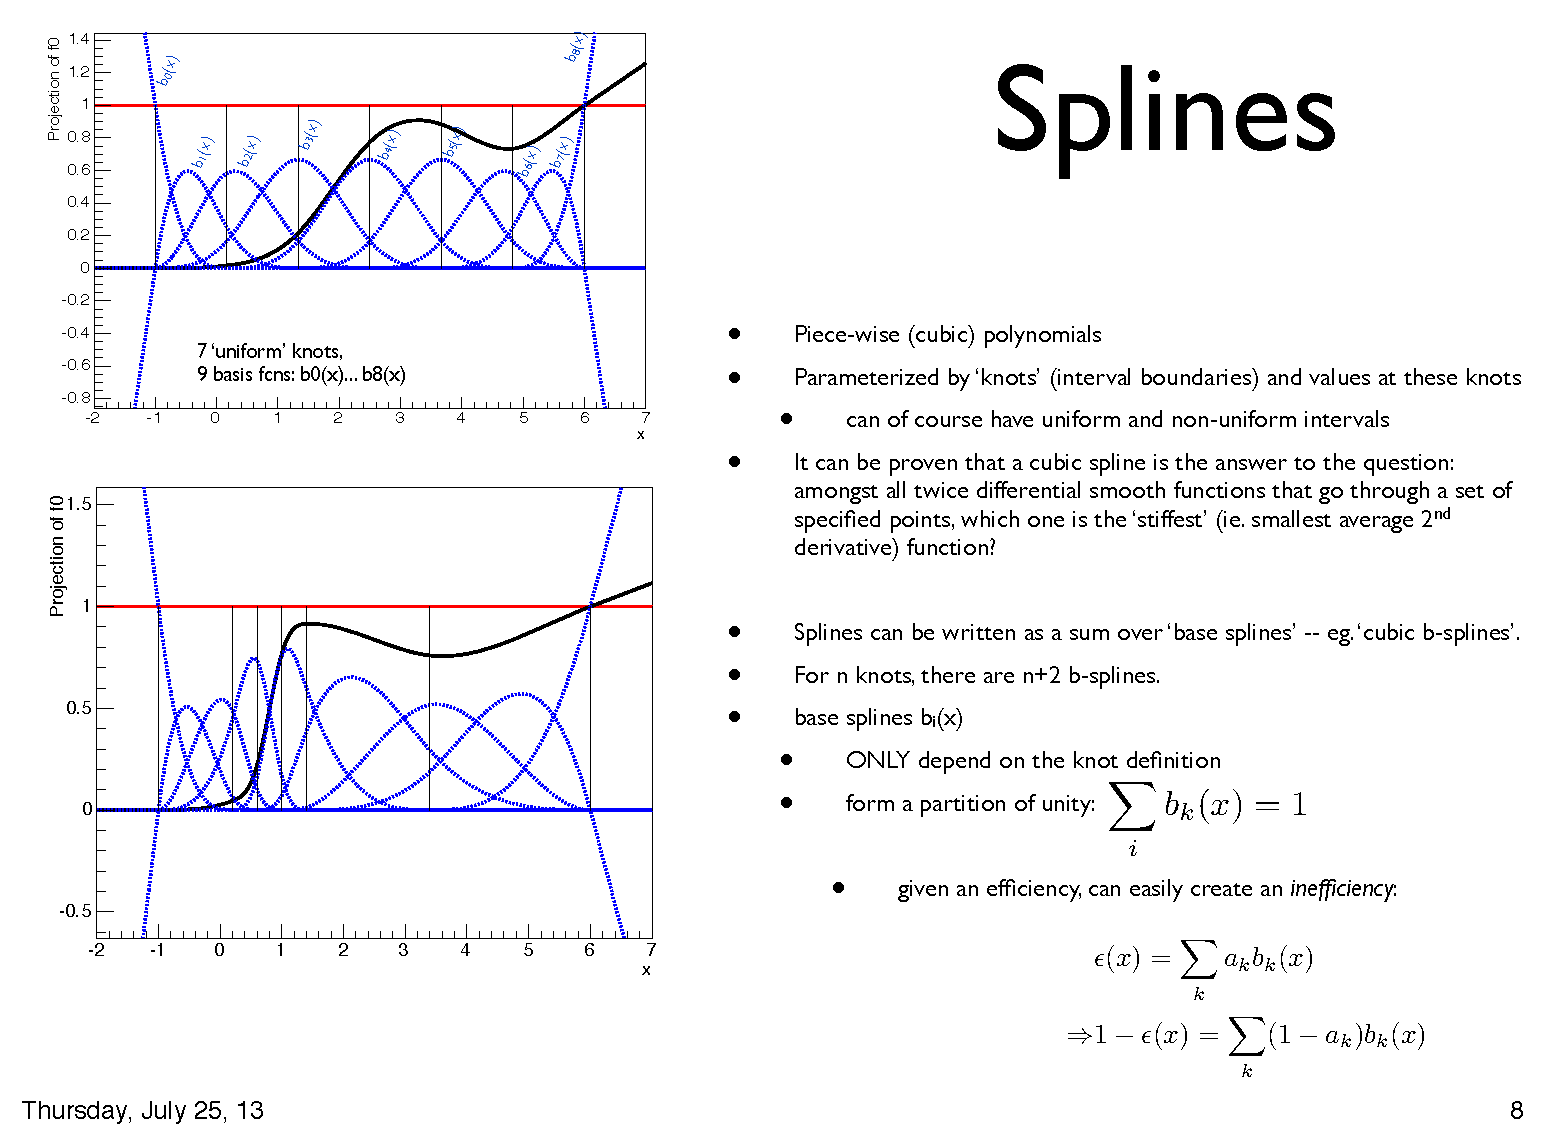
\includegraphics[width=.8\textwidth,clip]{splinebasics}
\rotatebox{90}{\tiny\color{gray} G. Raven, CP Tools and Techniques meeting, July 25th 2013}
\rotatebox{90}{\tiny\color{gray} M. Karbach, G. Raven, M. Schiller: LHCb-INT-2013-043}
\end{center}
\end{frame}

\begin{frame}[fragile]{1D splines as acceptance}
\begin{itemize}
\item define knots ($x_i$):
\begin{lstlisting}
time = RooRealVar('time', 'time', 0.2, 15.)
myknots = [ .2, .4, .6, .8, 1., 2., 3., 6., 12.]
knotbinning = RooBinning(time.getMin(), time.getMax(), 'knotbinning')
for v in myknots:
    knotbinning.addBoundary(v)
knotbinning.removeBoundary(time.getMax())
knotbinning.removeBoundary(time.getMin())
\end{lstlisting}
\item define spline coefficients
\begin{lstlisting}
coefflist = RooArgList()
for i in xrange(0, len(knots)):
    coefflist.addRooRealVar('SplineAccCoeff%u' % i, 'SplineAccCoeff%u' % i, coeffs[i], 0., 2.))
\end{lstlisting}
\item create the spline, and the resolution model from it
\begin{lstlisting}
tacc = RooCubicSplineFun('SplineAcceptance', 'SplineAcceptance', time, 'knotbinning', coefflist)
fit_resmodel = RooGaussEfficiencyModel('fit_resmodel', 'fit_resmodel', time, tacc, zero, timeerr, SF, SF)
\end{lstlisting}
\item that's it (essentially), can use this resolution-model-with-acceptance
    in RooFit classes like RooDecay, RooBDecay, \ldots
\end{itemize}
\end{frame}

\begin{frame}{1D splines for use as acceptance}
\begin{itemize}
\item there are a couple of stumbling stones (as usual):
\begin{itemize}
\item knot intervals must fully cover the fit range, and may not leak
    ``outside''
\item for generation, it's faster to use a {\tt RooEffProd} of the
    resolution-model-convolved {\tt RooBDecay} and the spline\\
\begin{itemize}
\item[$\rightarrow$] {\color{blue} different PDFs for generation and fitting!}
    \\
    (nice cross-check!)
\item if you want to generate toys, make sure your spline coefficients are all
    smaller than 1
\end{itemize}
\end{itemize}
\end{itemize}
\end{frame}

\begin{frame}{1D splines for use as acceptance}
\begin{itemize}
\item choose knot positions (more where curvature of acceptance is high)
\item can then fit spline coefficients to control channel/MC/\ldots
\item problems: \\
\begin{minipage}[b]{.47\textwidth}
\begin{itemize}
\item overall scale of spline not set: fix one coefficient to 1
\item at large times (low stats), tend to pick up stat. fluctuations, but
    expect uncurved acceptance \\
    {\color{blue} $\rightarrow$ fix last knot coefficient from linear
    extrapolation of previous two}
\end{itemize}
\end{minipage}
\begin{minipage}[b]{.45\textwidth}
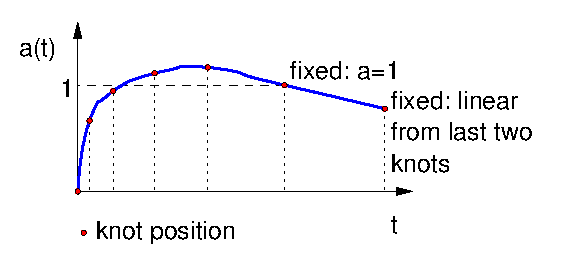
\includegraphics[width=.99\textwidth]{spline-fix}
\end{minipage}
\end{itemize}
\end{frame}

\begin{frame}[fragile]{1D splines for use as acceptance}
\begin{itemize}
\item naturally, this comes canned as a python routine:
\begin{lstlisting}[language=python]
from B2DXFitters.acceptanceutils import buildSplineAcceptance

# time range e.g. from 0.2 to 15 ps
acc, accnorm = buildSplineAcceptance(ws, time, 'Bs2DsK_acceptance',
    [ 0.5, 1.0, 1.5, 3.0, 6.0, 12.0 ], # knot positions
    [ 0., 0.5, 1.0, 1.0, 1.0, 1.0 ],   # initial coefficients (last two fixed, see last slide)
    True) # float spline coefficients in fit
\end{lstlisting}
\item {\tt acc} is an acceptance suitable for fitting
\item {\tt acc\_norm} is a normalised acceptance suitable for generation with
    {\tt RooEffProd} \\
    (applies overall scaling factor such that $a(t) < 1$ for all $t$)
\end{itemize}
$\,$ \hfill {\color{blue} $\rightarrow$ docs in {\tt
python/B2DXFitters/acceptanceutils.py}}
\end{frame}

\begin{frame}{spline systematics}
\begin{itemize}
\item this is always hard, but fortunately not very hard\ldots
\item for cubic splines, approximation error will be proportional to $\frac{\partial^4
    f(x)}{\partial x^4} \cdot h^4$ (h: spline subinterval size)
\item no need to calculate that: just try with twice the number of knots, and
    get estimate from the difference
\item if you're not stable, you likely have some problem with your
    approximation; plot to investigate
\end{itemize}
\end{frame}

\subsection{binned approximation}
\begin{frame}[fragile]{binned approximation}
\begin{itemize}
\item occasionally still useful:
\begin{itemize}
\item cross-checks
\item in other fits
\end{itemize}
\item two implementations:
\begin{itemize}
\item resolution-model based (just like splines - not cubic, but constant!):
    same use as splines, but use {\tt RooBinnedFun} instead of {\tt
    RooCubicSplineFun}
\item older implementation based on {\tt RooEffHistProd}, binning existing
    function as fast approximation
\begin{lstlisting}[language=python]
time = ... # RooRealVar for the time
acc = ... # some acceptance function
binning = RooUniformBinning(timelo, timehi, nbins, "someNameForBinning")
time.setBinning(binning, "someNameForBinning")
binned cc= RooBinnedPdf("name", "title", time, "someNameForBinnig", acc)
finalpdf = RooEffHistProd("name", "title", pdf_wo_acc, binnedacc)
\end{lstlisting}
\item[$\rightarrow$] also useful to avoid numerical integration in e.g. mass
    fits which are sculpted by some efficiency/threshold function\ldots
\end{itemize}
\end{itemize}
\end{frame}

\section{DecRateCoeff}
\begin{frame}{DecRateCoeff}
    \vfill
    $\,$ \hfill {\Huge DecRateCoeff} \hfill $\,$ \\
    \vfill
\end{frame}

\begin{frame}{DecRateCoeff}
\begin{itemize}
\item very versatile class
\item includes the tagging in RooBDecay
\item will therefore go slowly through the material
\begin{itemize}
\item average mistag
\item per-event mistag
\item asymmetries
\item advanced: combining taggers
\end{itemize}
\end{itemize}
\end{frame}

\subsection{average mistag}
\begin{frame}{DecRateCoeff: basics (1/3)}
\begin{itemize} \small
\item in $D_sK$, the pdf changes depending on final state charge ($q_f$) and
    tagging decision ($q_t$)
\item for average mistag $\omega$, the coefficient in front of e.g. the
    $\cos(\Delta m t)$ term is composed from contributions from $B_s$ and
    $\overline{B_s}$:
\begin{eqnarray*}
    C_{eff} &=& \sum_{q_i\in\{B,\overline{B}\}} P(q_f, q_t|q_i)\cdot
    C(q_i,q_f) \\
    & \sim & \left\{\begin{array}{l l}
    \epsilon_{tag}(C_f (1-\omega) + C_f (-\omega)) & q_t = +1,\, q_f = +1 \\
    \epsilon_{tag}(-C_f (-\omega) - C_f (1 - \omega)) & q_t = -1,\, q_f = +1 \\
    (1-\epsilon_{tag})(C_f - C_f)  & q_t = 0,\,  q_f = +1 \\
    (1-\epsilon_{tag})({\overline{C}_{\bar{f}}} - {\overline{C}_{\bar{f}}}) & q_t = 0,\,  q_f = -1 \\
    \epsilon_{tag}({\overline{C}_{\bar{f}}} (-\omega) + {\overline{C}_{\bar{f}}} (1
    -\omega)) & q_t = -1,\, q_f = -1 \\
    \epsilon_{tag}(-{\overline{C}_{\bar{f}}} (1-\omega) - {\overline{C}_{\bar{f}}}
    (-\omega)) & q_t = +1,\, q_f = -1 \\
\end{array}\right. \end{eqnarray*}
\item {\color{blue} make sure you recognise it as the formula we all know and
    love!}
\item it has (conceptually) a pdf inside, so it must \emph{normalise} itself
\end{itemize}
\end{frame}

\begin{frame}[fragile]{DecRateCoeff: average mistag}
\begin{itemize} \small
\item can play this game for
\begin{itemize}
\item CP-odd coefficients (for the $\sin/\cos(\Delta m t)$ terms): \\
    $C$ enters with sign of $q_i\cdot q_f$
\item CP-even coefficients (for the $\sinh/\cosh(\frac{\Delta \Gamma t}{2})$ terms): \\
    $C$ enters without sign
\end{itemize}
\item constructor:
\begin{lstlisting}[language=C++]
DecRateCoeff(const char* name, const char* title, Flags flags,
        RooAbsCategory& qf, RooAbsCategory& qt,
        RooAbsReal& Cf, RooAbsReal& Cfbar,
        RooAbsReal& tageff, RooAbsReal& eta,
        RooAbsReal& aprod, RooAbsReal& adet,
        RooAbsReal& atageff);
\end{lstlisting}
\item {\tt flags} can be {\tt CPEven} or {\tt CPOdd}
\item or {\tt | Minus} to it when you need an overall minus sign in front of
    $C$
\item if you want to fit
    $\overline{C} = (C_f+\overline{C}_{\bar{f}})/2$ and
    $\Delta C = (C_f-\overline{C}_{\bar{f}})/2$, or {\tt | AvgDelta}
\item put asymmetries to {\tt RooConstVar("zero", "zero", 0.)} if you don't
    need them
\end{itemize}
\end{frame}

\subsection{per-event mistag}
\begin{frame}{DecRateCoeff: basics (2/3)}
\begin{itemize} \small
    \item for (calibrated) per-event mistag $\omega(\eta)$, things become a little more complicated
\begin{eqnarray*}
    C_{eff} &=& \sum_{q_i\in\{B,\overline{B}\}} P(q_f, q_t|q_i) \cdot
    P(\eta|q_t)\cdot
    C(q_i,q_f) \\
    & \sim & \left\{\begin{array}{l l}
    \epsilon_{tag}P(\eta)(C_f (1-\omega(\eta)) + C_f (-\omega(\eta))) & q_t = +1,\, q_f = +1 \\
    \epsilon_{tag}P(\eta)(-C_f (-\omega(\eta)) - C_f (1 - \omega(\eta))) & q_t = -1,\, q_f = +1 \\
    (1-\epsilon_{tag})U(\eta)(C_f - C_f)  & q_t = 0,\,  q_f = +1 \\
    (1-\epsilon_{tag})U(\eta)({\overline{C}_{\bar{f}}} - {\overline{C}_{\bar{f}}}) & q_t = 0,\,  q_f = -1 \\
    \epsilon_{tag}P(\eta)({\overline{C}_{\bar{f}}} (-\omega(\eta)) + {\overline{C}_{\bar{f}}} (1
    -\omega(\eta))) & q_t = -1,\, q_f = -1 \\
    \epsilon_{tag}P(\eta)(-{\overline{C}_{\bar{f}}} (1-\omega(\eta)) - {\overline{C}_{\bar{f}}}
    (-\omega(\eta))) & q_t = +1,\, q_f = -1 \\
\end{array}\right. \end{eqnarray*}
\item $U(\eta)$ is a uniform distribution (whatever you set the mistag to for
    untagged events, you'll always get the same contribution)
\end{itemize}
\end{frame}

\begin{frame}[fragile]{DecRateCoeff: per-event mistag}
\begin{itemize} \small
\item same game
\item constructor:
\begin{lstlisting}[language=C++]
DecRateCoeff(const char* name, const char* title, Flags flags,
    RooAbsCategory& qf, RooAbsCategory& qt,
    RooAbsReal& Cf, RooAbsReal& Cfbar,
    RooAbsRealLValue& etaobs, RooAbsPdf& etapdf,
    RooAbsReal& tageff, RooAbsReal& eta,
    RooAbsReal& aprod, RooAbsReal& adet,
    RooAbsReal& atageff);
\end{lstlisting}
\item {\tt etaobs} is the observable $\eta$
\item {\tt etapdf} is $P(\eta)$
\item {\tt eta} is the calibrated mistag $\eta_c(\eta) = \omega(\eta)$
\end{itemize}
\end{frame}

\subsection{asymmetries}
\begin{frame}{DecRateCoeff: basics (3/3)}
\begin{itemize} \small
\item with asymmetries, this becomes even more complicated:
\begin{itemize}
\item $\epsilon_{tag}\rightarrow\epsilon_{tag}\cdot(1+q_ta_{tag})$
\item $\omega(\eta)\rightarrow\omega(\eta),\,\overline{\omega}(\eta)$
\item add factor $(1+q_ia_{prod})$ everywhere
\item add factor $(1+q_fa_{det})$ everywhere
\end{itemize}
\item full expression too large (and ugly) for slides, so see
\begin{itemize}
\item appendix to 1 fb$^{-1}$ $D_sK$ ANA note
\item doxygen docs for {\tt DecRateCoeff} ({\tt make doxy} in standalone)
\end{itemize}
\end{itemize}
\end{frame}

\begin{frame}[fragile]{DecRateCoeff: asymmetries}
\begin{itemize} \small
\item same game yet again
\item constructor:
\begin{lstlisting}[language=C++]
DecRateCoeff(const char* name, const char* title, Flags flags,
    RooAbsCategory& qf, RooAbsCategory& qt,
    RooAbsReal& Cf, RooAbsReal& Cfbar,
    RooAbsRealLValue& etaobs, RooAbsPdf& etapdf,
    RooAbsReal& tageff, RooAbsReal& eta, RooAbsReal& etabar,
    RooAbsReal& aprod, RooAbsReal& adet,
    RooAbsReal& atageff);
\end{lstlisting}
\item {\tt etaobs} is the observable $\eta$
\item {\tt etapdf} is $P(\eta)$
\item {\tt eta} is the calibrated mistag $\eta_c(\eta) = \omega(\eta)$ for $B$
\item {\tt etabar} is the calibrated mistag $\overline{\eta_c}(\eta) =
        \overline{\omega}(\eta)$ for
    $\overline{B}$
\end{itemize}
\end{frame}

\subsection{combining taggers}
\begin{frame}{DecRateCoeff: extra: combining taggers (1/7)}
\begin{itemize}
\item in principle, one can write down the fromulae on the past few slides for
    more than one tagger
\begin{itemize}
\item that would (correctly) combine multiple taggers within {\tt DecRateCoeff}
\item rewrite in progress, but not ready for production yet
\end{itemize}
\item I had hoped to be faster to avoid what follows, but\ldots
\item combining taggers workaround, required steps:
\begin{itemize}
\item split into three mutually exclusive taggers ($|qt|=$ 1 for OS, 2 for
    SSK, 3 for both OS+SSK)
\item calibrate taggers as preprocessing step with average $p_0, p_1$, mangle tagging decision (last
    item)
\item run toy to propagate asymmetries and errors on calibration to calibrated
    mistag
\item fit with six calibrations, one for each tagger and true B flavour
\item constrain the various $p_0, p_1$ according to result of toys
\end{itemize}
\end{itemize}
\end{frame}

\begin{frame}[fragile]{DecRateCoeff: extra: combining taggers (2/7)}
\begin{itemize}
\item step 1: tuple preprocessing
\begin{itemize}
\item suppose you have a RooDataset with your data somewhere
\item use these steps to add two new variables to it:
\begin{lstlisting}[language=Python]
import MistagCalibration, DLLTagCombiner, TagDLLToTagEta, TagDLLToTagDec, RooArgList

# uncalibrated mistags eta_OS, eta_SSK, decisions qt_OS, qt_SSK; there are part of data set
# calibration constants are p0_OS, p1_OS, etaavg_OS, similar for SSK
eta_OSc = WS(ws, MistagCalibration('eta_OSc', 'eta_OSc', eta_OS, p0_OS, p1_OS, etaavg_OS))
eta_SSKc = WS(ws, MistagCalibration('eta_SSKc', 'eta_SSKc', eta_SSK, p0_SSK, p1_SSK, etaavg_SSK))
qts = RooArgList(qt_OS, qt_SSK)
etas = RooArgList(eta_OSc, eta_SSKc)
dll = WS(ws, DLLTagCombiner('dlltag', 'dlltag', qts, etas))
eta = WS(ws, TagDLLToTagEta('eta', 'eta', dll))
qt = WS(ws, TagDLLToTagDec('qt', 'qt', dll, qts))

# add to data set
dataset.addColumn(eta)
dataset.addColumn(qt)
\end{lstlisting}
\item then save the data set to a new workspace
\end{itemize}
\item if you prefer to work with straight tuples, have a look at {\tt
    TagCombiner.h}
\end{itemize}
\end{frame}

\begin{frame}[fragile]{DecRateCoeff: extra: combining taggers (3/7)}
\begin{itemize}
\item step 2a: work out correction for calibration asymmetries
\begin{itemize}
\item in step 1, we apply average correction for $B/\overline{B}$
\item not correct yet, so correct remaining discrepancy in fit
\item use toy to figure out the post-combination calibration asymmetries
    (is exact for linear calibration polynomials)
\item {\tt standalone/taggingtoy/tagcomb.cc} contains the code
\begin{enumerate}
\item generates events with correct calibration for $B/\overline{B}$, and OS
    and SSK \\
    (mistag templates from ROOT file, just splot your tuple after mass fit)
\item combines using average calibration for OS and SSK
\item recalibrates output separately for ($B,\overline{B}$)x(OS only, SSK
    only, OS+SSK)
\item use to figure out post-combination calibrations, and correlations
\end{enumerate}
\item you get six sets of calibration constants, which are all correlated
    among each other, see next slide
\end{itemize}
\end{itemize}
\end{frame}

\begin{frame}[fragile]{DecRateCoeff: extra: combining taggers (4/7)}
    \vspace{-3mm}
\begin{itemize}
\item step 2b: work out correction for calibration asymmetries
\item {\tt make tagcomb; ./tagcomb} (eventually) prints
\begin{lstlisting}[language=sh]
[... much output ...]
Total calibration:
B    OS only : eta_c = 0.376730+/-0.004389 + (1.048155+/-0.039917) * (eta - 0.371147) --- correl(p0, p1) = -0.111791
B    SSK only: eta_c = 0.404896+/-0.011412 + (0.995879+/-0.148797) * (eta - 0.414892) --- correl(p0, p1) = -0.122611
B    OS + SSK: eta_c = 0.338363+/-0.005959 + (1.027861+/-0.038725) * (eta - 0.338493) --- correl(p0, p1) = -0.874463
Bbar OS only : eta_c = 0.365517+/-0.004395 + (0.950216+/-0.040072) * (eta - 0.371147) --- correl(p0, p1) = -0.111883
Bbar SSK only: eta_c = 0.424801+/-0.011414 + (1.004340+/-0.150355) * (eta - 0.414892) --- correl(p0, p1) = -0.123455
Bbar OS + SSK: eta_c = 0.338781+/-0.006030 + (0.971845+/-0.039962) * (eta - 0.338493) --- correl(p0, p1) = -0.878334

Correlations:
          0        1        2        3        4        5        6        7        8        9       10       11
 0  1.00000 -0.11179  0.00000  0.00000  0.49565 -0.12126  0.88340 -0.09034  0.00000  0.00000  0.43630 -0.11593
 1 -0.11179  1.00000  0.00000  0.00000 -0.17072  0.36865 -0.09043  0.80830  0.00000  0.00000 -0.13861  0.30321
 2  0.00000  0.00000  1.00000 -0.12261  0.65815 -0.54123  0.00000  0.00000  0.93878 -0.12029  0.63338 -0.52537
 3  0.00000  0.00000 -0.12261  1.00000 -0.63105  0.81198  0.00000  0.00000 -0.12244  0.98640 -0.60841  0.78788
 4  0.49565 -0.17072  0.65815 -0.63105  1.00000 -0.87446  0.43682 -0.13789  0.62212 -0.62217  0.94027 -0.84147
 5 -0.12126  0.36865 -0.54123  0.81198 -0.87446  1.00000 -0.10427  0.29779 -0.51403  0.80069 -0.83010  0.95060
 6  0.88340 -0.09043  0.00000  0.00000  0.43682 -0.10427  1.00000 -0.11188  0.00000  0.00000  0.49475 -0.13419
 7 -0.09034  0.80830  0.00000  0.00000 -0.13789  0.29779 -0.11188  1.00000  0.00000  0.00000 -0.17092  0.37480
 8  0.00000  0.00000  0.93878 -0.12244  0.62212 -0.51403  0.00000  0.00000  1.00000 -0.12345  0.67273 -0.55661
 9  0.00000  0.00000 -0.12029  0.98640 -0.62217  0.80069  0.00000  0.00000 -0.12345  1.00000 -0.61649  0.79852
10  0.43630 -0.13861  0.63338 -0.60841  0.94027 -0.83010  0.49475 -0.17092  0.67273 -0.61649  1.00000 -0.87833
11 -0.11593  0.30321 -0.52537  0.78788 -0.84147  0.95060 -0.13419  0.37480 -0.55661  0.79852 -0.87833  1.00000
\end{lstlisting}
\item this includes contributions from combination, stat. and syst. errors
\item corresponding tables exist earlier in the output for \\
\begin{minipage}{.4\textwidth}
\begin{itemize}
\item combination only
\item combination + stat. error
\end{itemize}
\end{minipage}
\begin{minipage}{.4\textwidth}
\begin{itemize}
\item combination + syst. error
\item (total error)
\end{itemize}
\end{minipage}
\end{itemize}
\end{frame}

\begin{frame}[fragile]{DecRateCoeff: extra: combining taggers (5/7)}
\begin{itemize}
\item step 2b: work out tagging efficiency asymmetries post combination
\begin{itemize}
\item splitting OS and SSK taggers into OS only, SSK only and OS+SSK changes
    the tagging efficiencies and asymmetries for the three ``new taggers''
\item look at {\tt standalone/taggingtoy/eps.c} to see how to calculate it
\begin{lstlisting}[language=sh]
> make eps; ./eps
Combining tagging efficiencies (signal):
 OS: eps = 0.387000+/-0.003000 Delta eps = -0.001970+/-0.001260
SSK: eps = 0.477000+/-0.003000 Delta eps =  0.000220+/-0.000040

 OS only: eps=0.202401+/-0.001952 a=-0.002756+/-0.001628
SSK only: eps=0.292401+/-0.002330 a= 0.001837+/-0.001029
  OS+SSK: eps=0.184599+/-0.001843 a=-0.002315+/-0.001629

Correlation:
   1.00000000e+00  -9.63105978e-01   2.49481592e-01   1.01449534e-02   7.02032244e-03   1.02339761e-02
  -9.63105978e-01   1.00000000e+00   2.03354154e-02  -8.05565545e-03  -5.77788479e-03  -8.17299797e-03
   2.49481592e-01   2.03354154e-02   1.00000000e+00   8.98034829e-03   5.01061453e-03   8.88495266e-03
   1.01449534e-02  -8.05565545e-03   8.98034829e-03   1.00000000e+00  -9.99652998e-01   9.98788285e-01
   7.02032244e-03  -5.77788479e-03   5.01061453e-03  -9.99652998e-01   1.00000000e+00  -9.97590361e-01
   1.02339764e-02  -8.17299794e-03   8.88495268e-03   9.98788284e-01  -9.97590361e-01   1.00000000e+00
\end{lstlisting}
\end{itemize}
\item correlation matrix ordered
    ($\epsilon_{OS},\epsilon_{SSK},\epsilon_{OS+SSK},a_{OS}, a_{SSK},
    a_{OS+SSK}$)
\end{itemize}
\end{frame}

\begin{frame}[fragile]{DecRateCoeff: extra: combining taggers (6/7)}
\begin{itemize}
\item step 3: set up fit
\begin{itemize}
\item get mistag templates for the three taggers (OS only, SSK only, OS+SSK)
    from the data added in step 1
\item use constants for six calibrations from step 2a
\item use tagging efficiencies and asymmetries from step 2b
\item set up constraints for calibration constants (12D) and tagging
    efficiencies and asymmetries (6D), see next slide
\item then, use this DecRateCoeff constructor:
\begin{lstlisting}[language=C++]
DecRateCoeff(const char* name, const char* title, Flags flags,
    RooAbsCategory& qf, RooAbsCategory& qt,
    RooAbsReal& Cf, RooAbsReal& Cfbar,
    RooAbsRealLValue& etaobs, RooArgList& etapdfs,
    RooArgList& tageffs, RooArgList& etas, RooArgList& etabars,
    RooAbsReal& aprod, RooAbsReal& adet,
    RooArgList& atageffs);
\end{lstlisting}
\item same as before, RooArgLists are ordered OS only, SSK only, OS+SSK
\end{itemize}
\end{itemize}
\end{frame}

\begin{frame}[fragile]{DecRateCoeff: extra: combining taggers (7/7)}
\begin{itemize}
\item what remains is to show how to construct the 6D or 12D constraints
\item numerially tricky, since cov. matrices damn near singular
\item special routine which can recover\ldots
\begin{lstlisting}[language=Python]
from B2DXFitters.GaussianConstraintBuilder import GaussianConstraintBuilder
cbuilder = GaussianConstraintBuilder(ws, {
    'GammaLb': 0.006, # constrain GammaLb to within 0.006
    # constrain S+Sbar, S-Sbar for Bd2DPi from PDG values (name: [ 'formula', [params], mean, error ])
    'Bd2DPi_avgSSbar': [ '0.5*(@0+@1)', ['Bd2DPi_S', 'Bd2DPi_Sbar'], +0.046, 0.023 ],
    'Bd2DPi_difSSbar': [ '0.5*(@0-@1)', ['Bd2DPi_S', 'Bd2DPi_Sbar'], -0.022, 0.021 ],
    'multivar_Bs2DsPiTagEffAsyms': [ # name: multivar_something
        # list of variables
        [ 'Bs2DsPi_TagEff0', 'Bs2DsPi_TagEff1', 'Bs2DsPi_TagEff2',
          'Bs2DsPi_AsymTagEff0', 'Bs2DsPi_AsymTagEff1', 'Bs2DsPi_AsymTagEff2' ],
        # errors
        [ 0.001952, 0.002330, 0.001843, 0.001628, 0.001029, 0.001629 ],
        # correlation matrix (always give full precision - only shortened here to fit on slide!)
        [ [  1.00000000e+00, -9.63105978e-01, 2.49481592e-01,  1.01449534e-02,  7.02032244e-03,  1.02339764e-02 ],
          [ -9.63105978e-01,  1.00000000e+00, 2.03354154e-02, -8.05565545e-03, -5.77788479e-03, -8.17299794e-03 ],
          [  2.49481592e-01,  2.03354154e-02, 1.00000000e+00,  8.98034829e-03,  5.01061453e-03,  8.88495268e-03 ],
          [  1.01449534e-02, -8.05565545e-03, 8.98034829e-03,  1.00000000e+00, -9.99652998e-01,  9.98788284e-01 ],
          [  7.02032244e-03, -5.77788479e-03, 5.01061453e-03, -9.99652998e-01,  1.00000000e+00, -9.97590361e-01 ],
          [  1.02339764e-02, -8.17299794e-03, 8.88495268e-03,  9.98788284e-01, -9.97590361e-01,  1.00000000e+00 ], ],
      ]
      # any other constraints you may have
  })
# get RooArgSet for use with fitTo's RooFit.ExternalConstraints option
constraints = cbuilder.getSetOfConstraints()
\end{lstlisting}
\item very useful to handle all your constraint needs (config dictionary!)
\end{itemize}
\end{frame}

\section{resolution model}
\begin{frame}{resolution model}
    \vfill
    $\,$ \hfill {\Huge resolution model} \hfill $\,$ \\
    \vfill
\end{frame}

\section{resolution model, k factors}
\begin{frame}{resolution model, k-factors}
\begin{itemize}
\item three big subtopics:
\begin{itemize}
\item obtaining resolution model
\item considerations for a fast fit
\item k-factors (partially reconstructed/misIDed modes)
\end{itemize}
\end{itemize}
\end{frame}

\subsection{obtaining a resolution model}
\begin{frame}[fragile]{obtaining a resolution model}
\begin{itemize}
\item easy, here are examples:
\begin{lstlisting}[language=Python]
from B2DXFitters.resmodelutils import getResolutionModel
config = {
    'DecayTimeResolutionModel': 'GaussianWithPEDTE',
    'DecayTimeResolutionBias': 0.,              # if there is a shift
    'DecayTimeResolutionScaleFactor': 1.15,     # usually the errors need a bit of scaling
    'Acceptance': 'Spline',                     # has to work closely with spline acceptance classes
    'Context':  'GEN' # or 'FIT', as the case may be
    }
# time is decay time variable, timeerr is decay time error

# get spline acceptance from somewhere
acc = #...
resmodel, acc = getResolutionModel(ws, config, time, timeerr, acc)
\end{lstlisting}
\item when you need an average decay time, use
\begin{lstlisting}[language=Python]
config = {
    'DecayTimeResolutionModel': {
        'sigmas': [sigma_1, sigma_2, ..., sigma_N],
        'fractions': [f_1, f_2, ..., f_N-1 ] } # non-recursive, i.e. add up to 100 %
    }
\end{lstlisting}
\item you can use {\tt scripts/AvgResModel.py} to fit the widths and fractions
    from a decay time error distribution
\end{itemize}
$\,$ \hfill {\color{blue}$\rightarrow$ see docs in {\tt
python/B2DXFitters/resmodelutils.py}}
\end{frame}

\subsection{considerations for a fast fit}
\begin{frame}[fragile]{considerations for a fast fit (1/2)}
\begin{itemize}
\item with per-event time errors, we get
    \[ P(t')\otimes G(t-t'|\sigma_t) \cdot P(\sigma_t) \]
\item[$\rightarrow$] {\color{blue}
        recalculation of normalisation $I(\sigma_t)=\int dt\, P(t')\otimes G(t-t'|\sigma_t)$ for every
    single event!}
\item despite analytical normalisation of convolution integral: SLOOOOOW!
\item however, $I(\sigma_t)$ varies slowly with $\sigma_t$
\begin{center}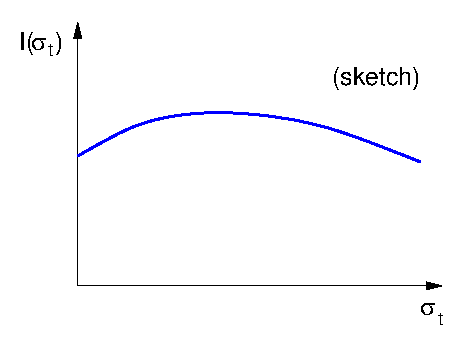
\includegraphics[width=.3\textwidth]{Isigmat} \end{center}
\item[$\rightarrow$] can tabulate in 100 points, and interpolate in between
    (fast!)
\end{itemize}
\end{frame}

\begin{frame}[fragile]{considerations for a fast fit (2/2)}
\begin{itemize}
\item need to tell RooFit to use the interpolation trick:
\begin{lstlisting}[language=Python]
from B2DXFitters.timepdfutils import parameteriseResModelIntegrals

config = { # tell how many bins in time error we need for table that's accurate enough
    'NBinsProperTimeError': 100
    }
# make it so!
parameteriseResModelIntegrals(config, ws, timeerrpdf, timeerr, resmodel)
\end{lstlisting}
\item will mostly be handled by {\tt buildBDecayTimePdf}
\end{itemize}
$\,$ \hfill {\color{blue}$\rightarrow$ see docs in {\tt
python/B2DXFitters/timepdfutils.py}}
\end{frame}

\subsection{k-factors}
\begin{frame}{k-factors (1/3)}
\vspace{-3mm}
\begin{itemize}
\item lifetime is calculated along the lines of
    $t=|\vec{x}_{SV}-\vec{x}_{PV}| \frac{m_{B_s}}{|\vec{p}|}$
\item for partially reconstructed and misid'ed modes, we get
    $\frac{m_{B_s}}{|\vec{p}|}$ wrong
\item idea: take correction factor from MC:
    \[ k =
    \frac{(m_{B_s}/|\vec{p}|)_{true}}{(m_{B_s}/|\vec{p}|)_{reco}}\]
\item can correct by substitution $t\longrightarrow k\cdot t$
\end{itemize}
\vspace{-3mm}
\begin{center}
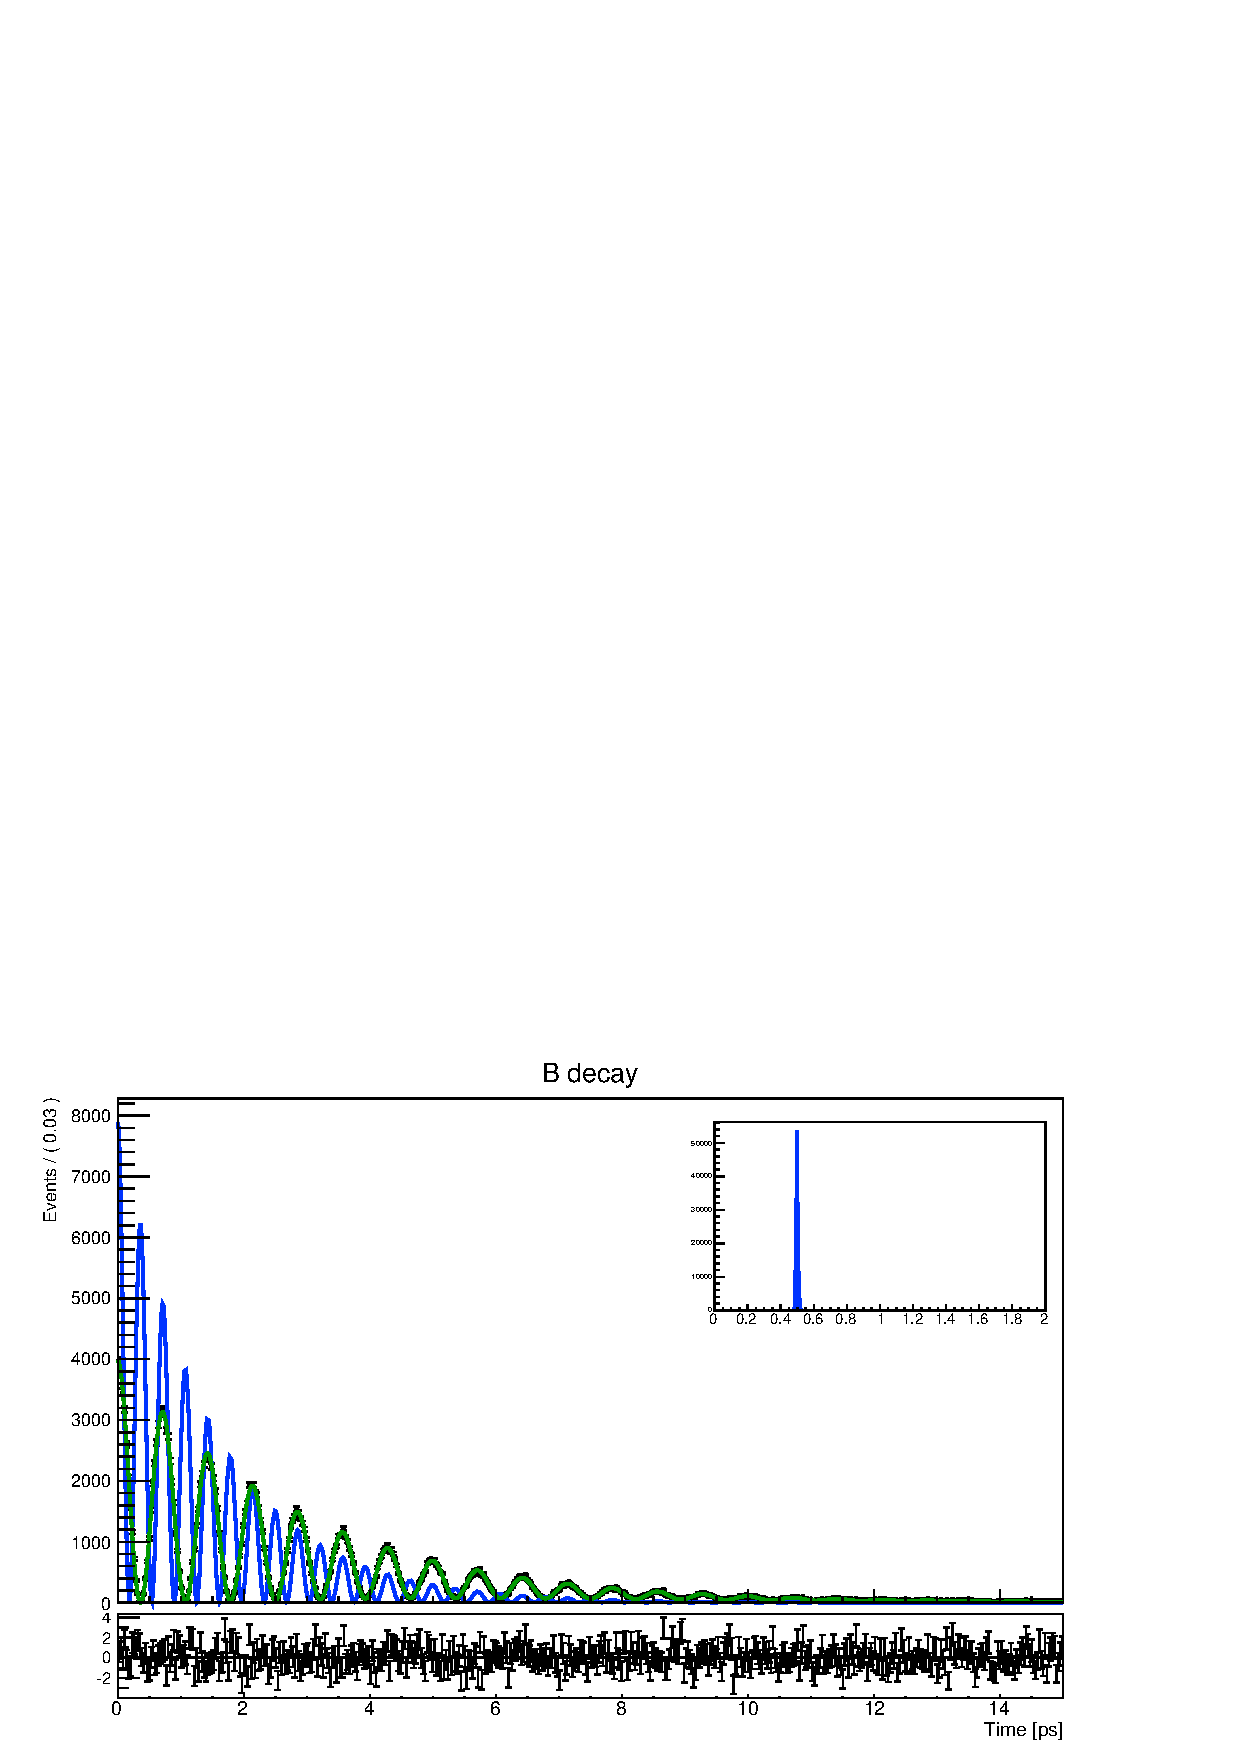
\includegraphics[width=.49\textwidth,clip]{kfactor-test0}
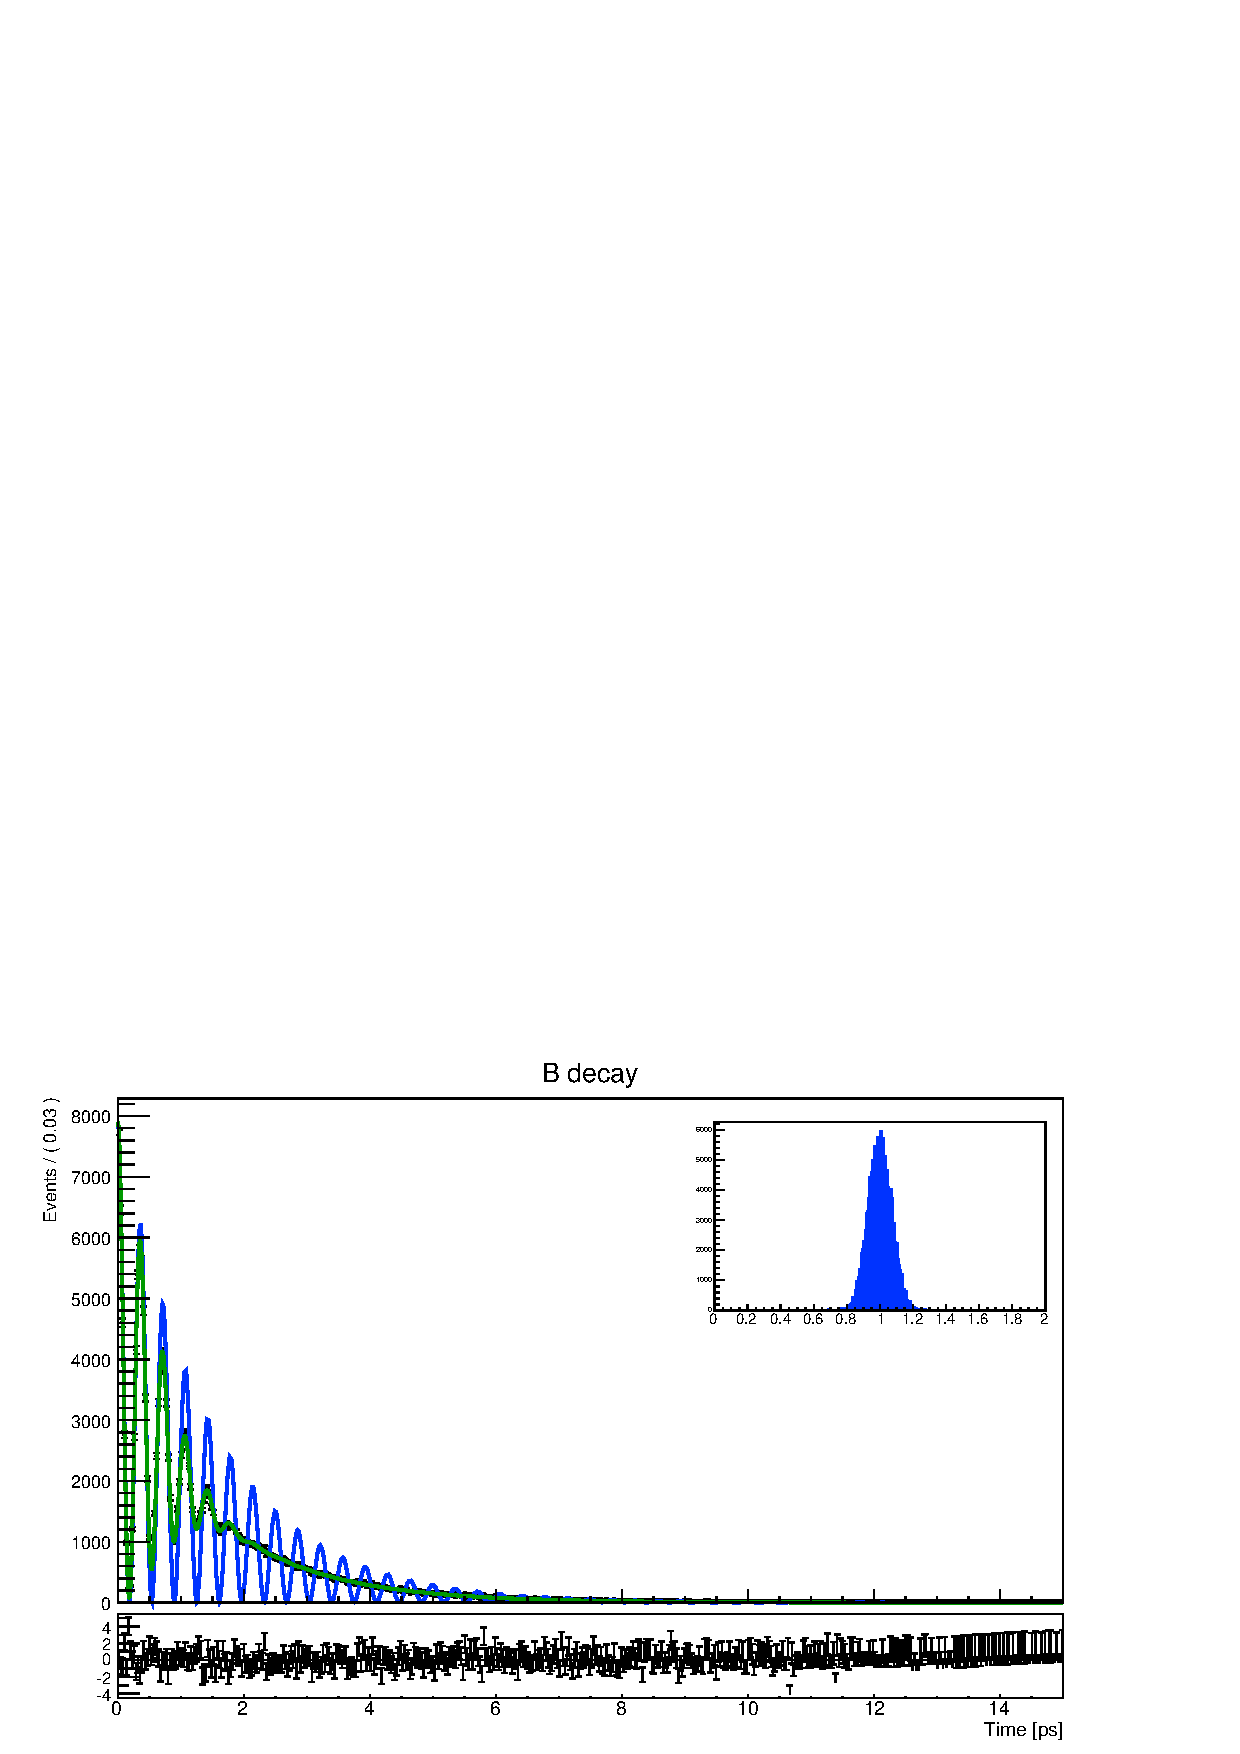
\includegraphics[width=.49\textwidth,clip]{kfactor-test1}
\rotatebox{90}{\tiny\color{gray}plots: Suvayu Ali}
\end{center}
\end{frame}

\begin{frame}{k-factors (2/3)}
\vspace{-3mm}
\begin{center}
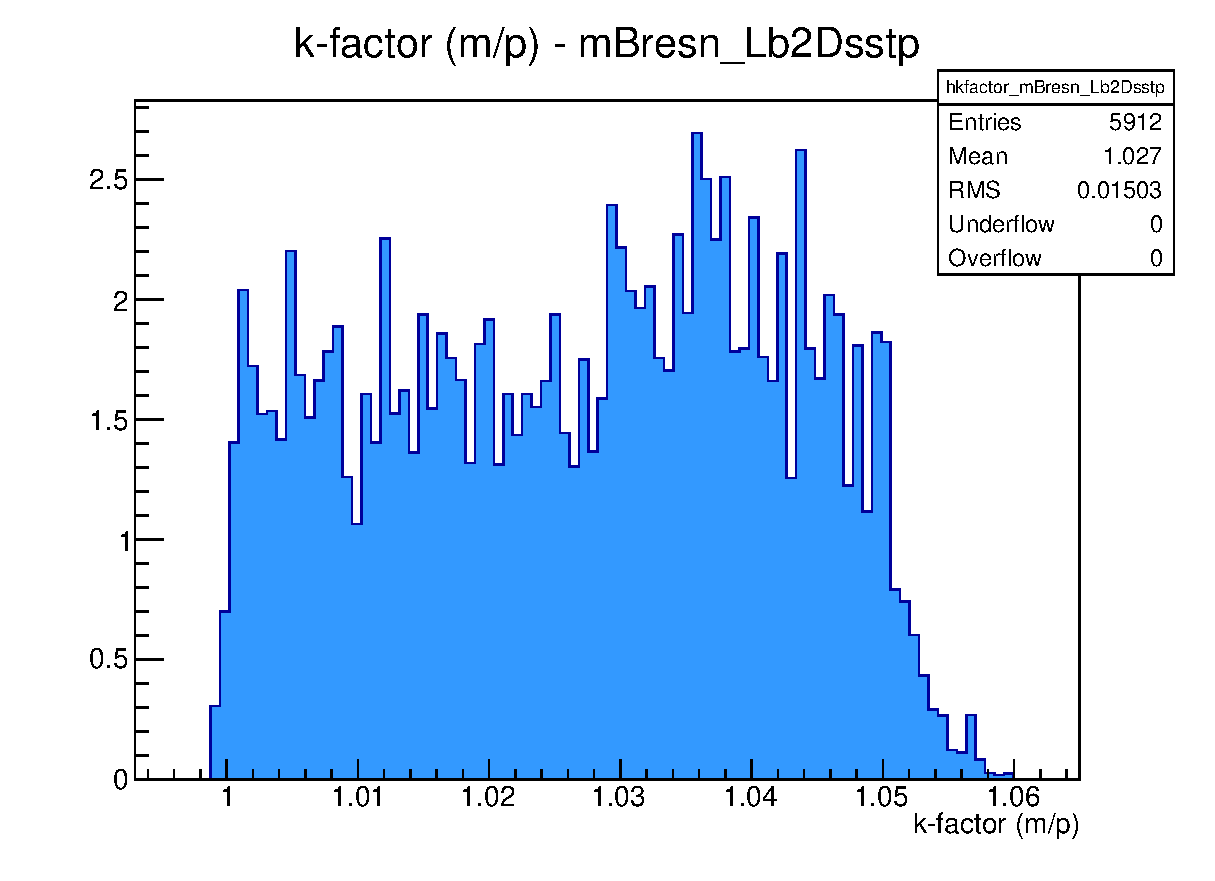
\includegraphics[width=.2425\textwidth]{kfactor-template-1}
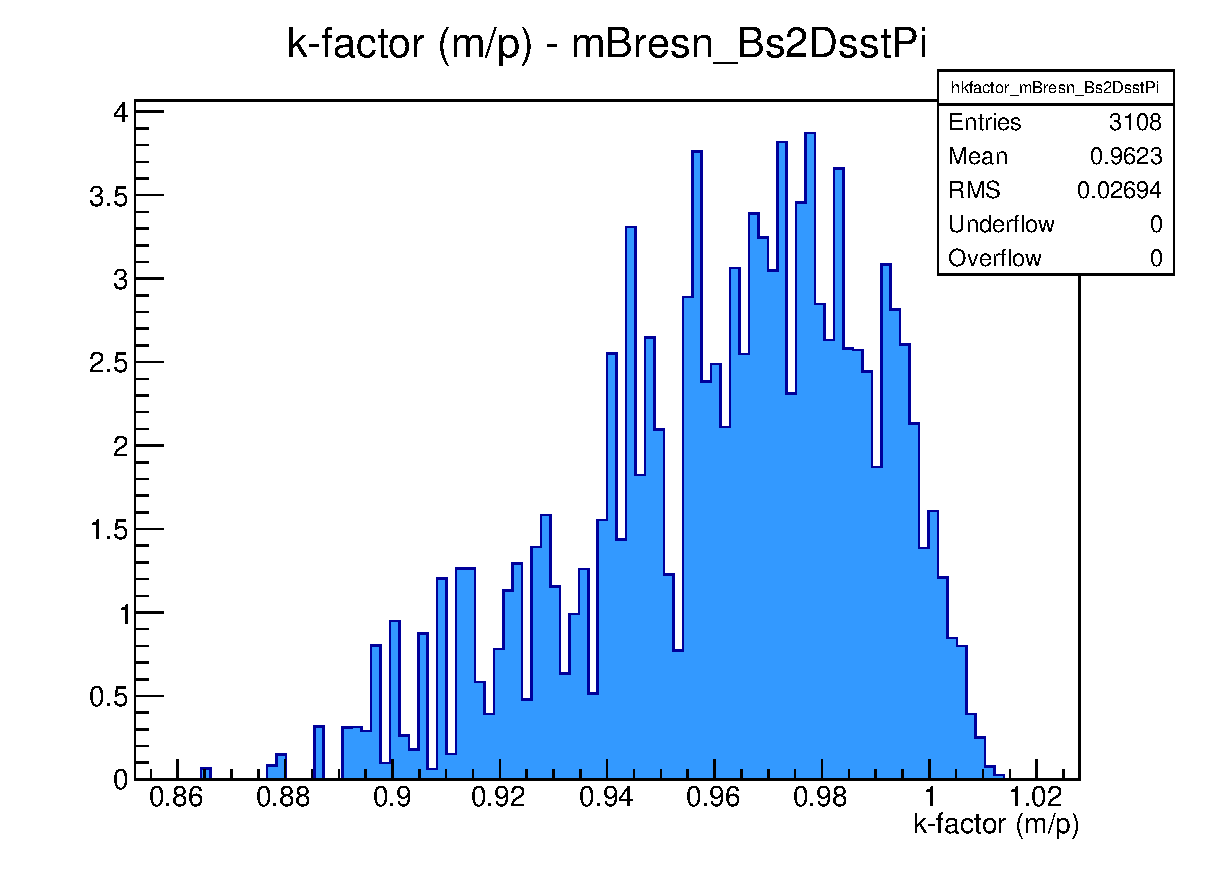
\includegraphics[width=.2425\textwidth]{kfactor-template-4}
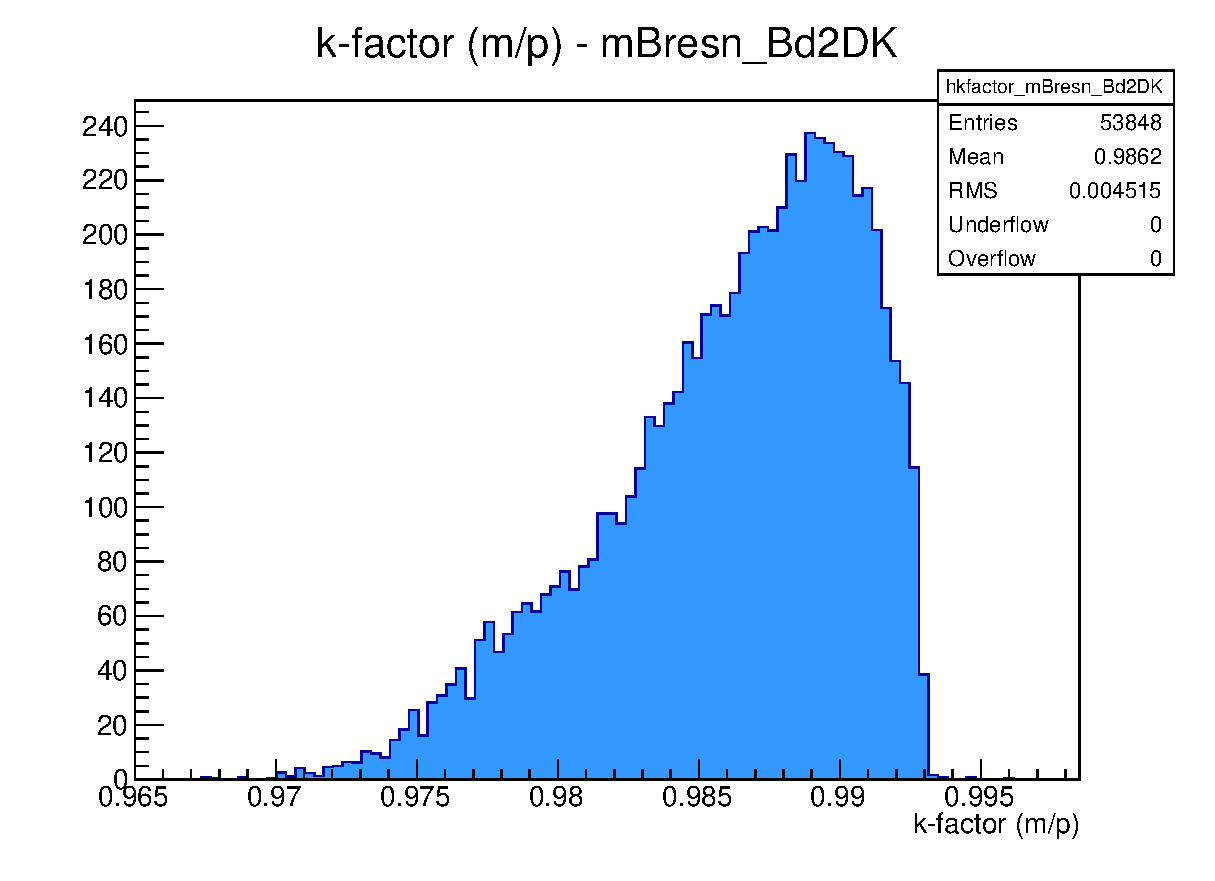
\includegraphics[width=.2425\textwidth]{kfactor-template-7}
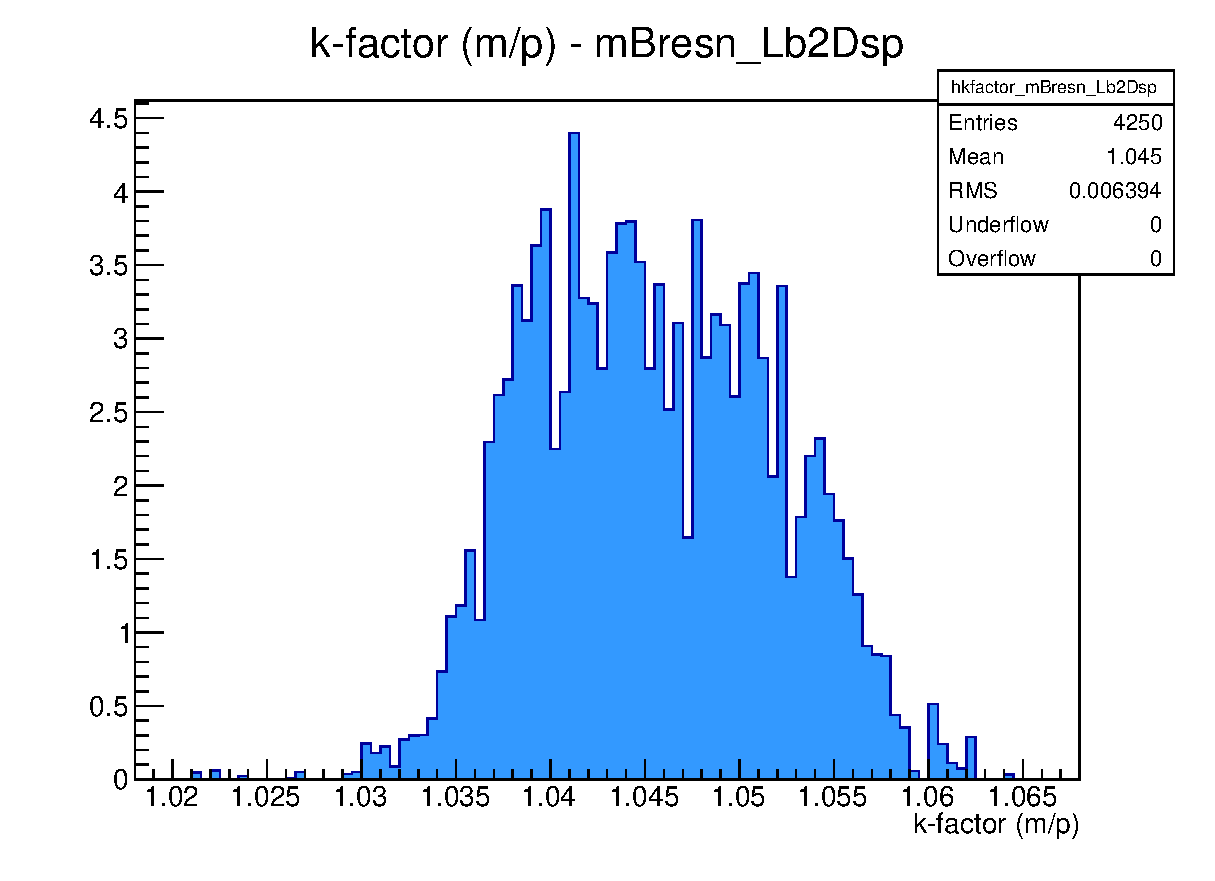
\includegraphics[width=.2425\textwidth]{kfactor-template-10} \\
\includegraphics[width=.2425\textwidth]{kfactor-template-13}
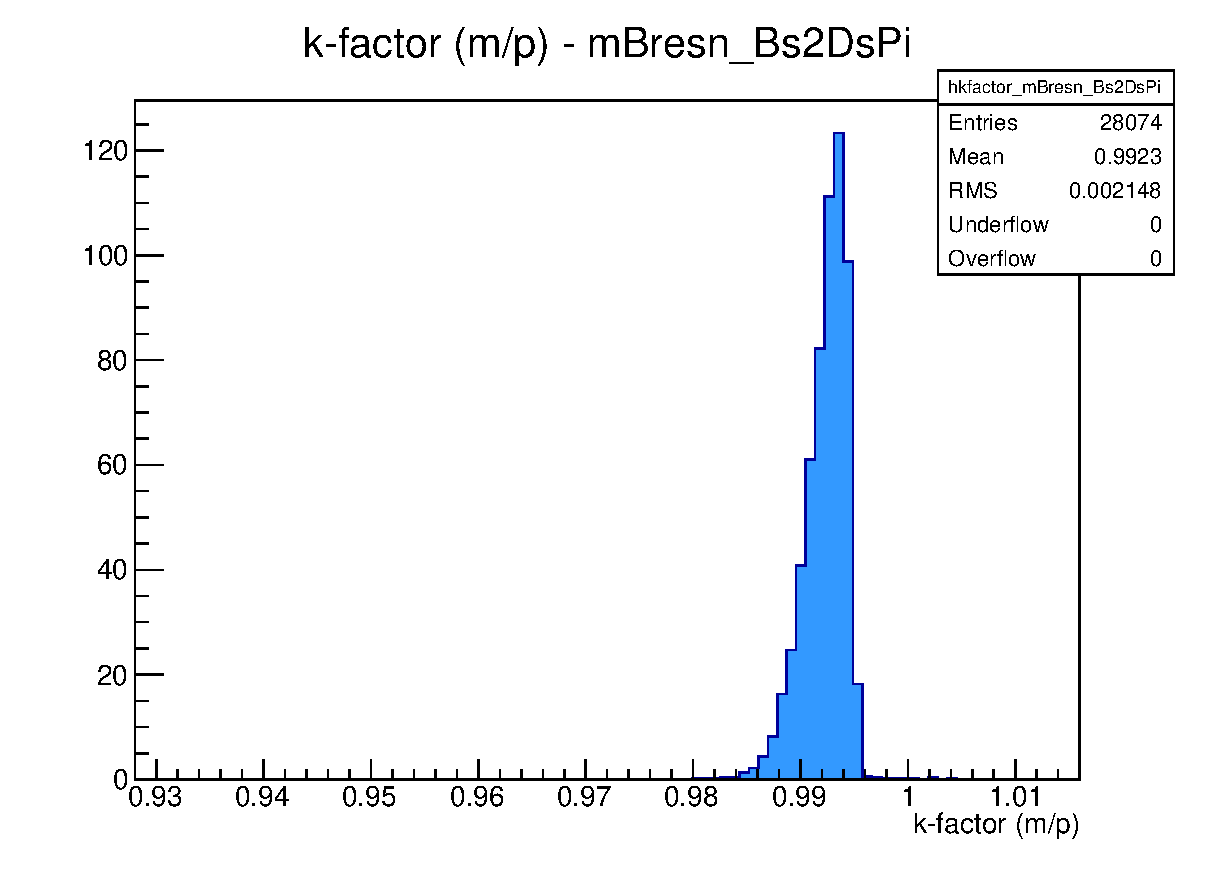
\includegraphics[width=.2425\textwidth]{kfactor-template-16}
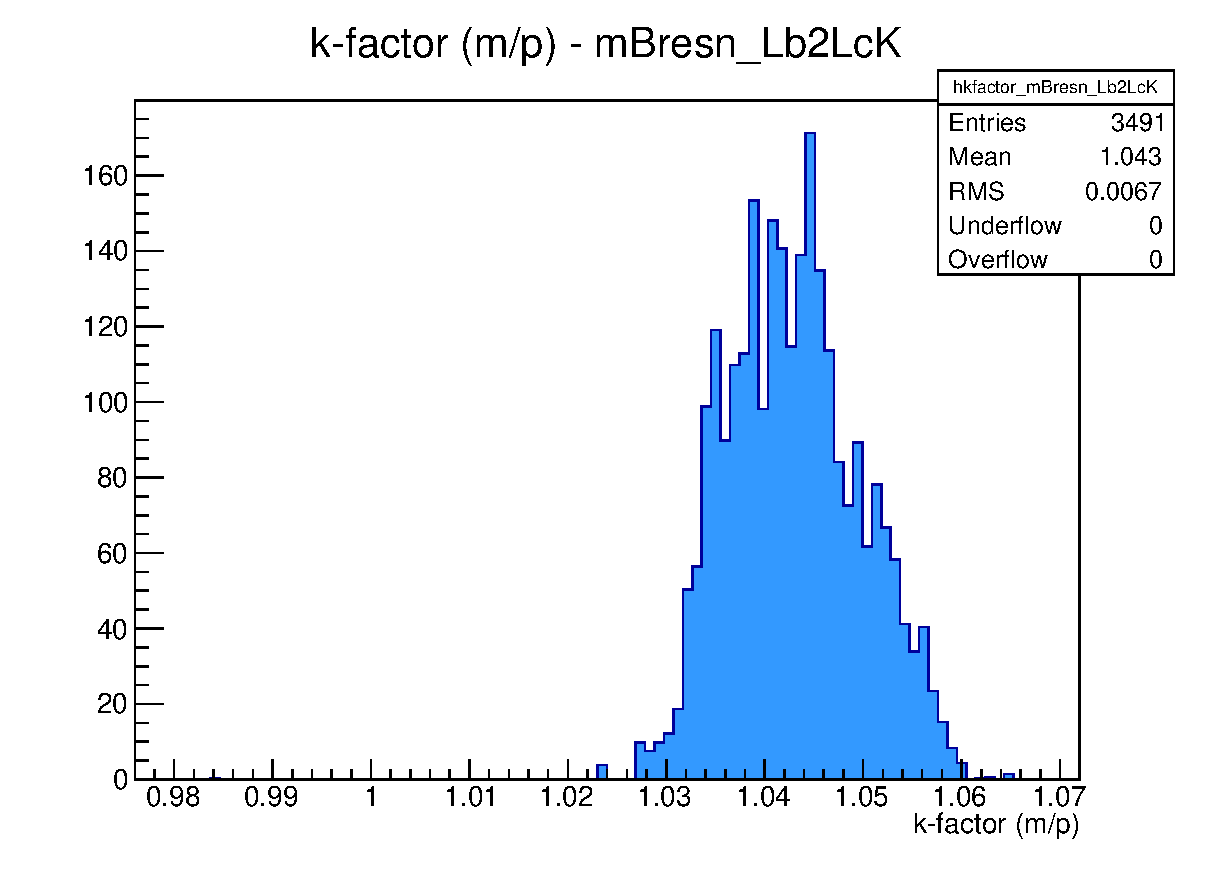
\includegraphics[width=.2425\textwidth]{kfactor-template-19}
\rotatebox{90}{\tiny\color{gray}plots: Suvayu Ali}
\end{center}
\vspace{-3mm}
\begin{itemize}
\item can now put this into toy generator(s) for $D_sK$
\item can also use it in cFit to get the BG description correct:
    \[ \frac{d\Gamma}{dt}(t; \Gamma, \Delta\Gamma, \Delta m) \longrightarrow
	\int d{\color{blue}k}\, P({\color{blue}k}) \cdot \frac{d\Gamma}{dt}(t;
    {\color{blue}k}\Gamma, {\color{blue}k}\Delta\Gamma, {\color{blue}k}\Delta
    m) \]
\end{itemize}
\end{frame}

\begin{frame}[fragile]{k-factors (3/3)}
\vspace{-3mm}
\begin{itemize}
\item convenient to express k-factor smearing as resolution model: {\tt
    RooKResModel}
\begin{itemize}
\item average correction for each event can be precalculated and cached
\end{itemize}
\begin{lstlisting}[language=Python]
from B2DXFitters.timepdfutils import applyKFactorSmearing

config = {
    'NBinsTimeKFactor': 100, # use 100 bins to bin k-factor distributions
    }
# time          - decay time observable
# timeresmodel  - resolution model (after applying spline acceptance)
# kvar          - k-factor variable (unobservable!)
# kfactorpdf    - k-factor distribution for mode
# last argument: list of targets { t_i } for substitution t_i -> k * t_i

# update timeresmodel to include k-factor smearing
timeresmodel = applyKFactorSmearing(config, ws, time, timeresmodel, kvar, kfactorpdf, [ Gamma, DeltaGamma, DeltaM ])
\end{lstlisting}
\item will mostly be handled by {\tt buildBDecayTimePdf}
\end{itemize}
$\,$ \hfill {\color{blue}$\rightarrow$ see docs in {\tt
python/B2DXFitters/timepdfutils.py}}
\end{frame}

\section{python, RooFit and ownership}
\begin{frame}{python, RooFit and ownership}
    \vfill
    $\,$ \hfill {\Huge python, RooFit} \hfill $\,$ \\
    $\,$ \hfill {\Huge and ownership} \hfill $\,$ \\
    \vfill
\end{frame}

\begin{frame}[fragile]{python, RooFit and ownership}
\begin{itemize}
\item python's objects are \emph{reference-counted}
\begin{itemize}
\item no need for memory management
\end{itemize}
\item C++/RooFit uses explicit memory management
\begin{itemize}
\item need \lstinline!new/delete!
\item ownership transfer often not clear in ROOT/RooFit \\
    (ownership: which code is responsible for calling delete)
\item worse: RooFit clones objects all over the place\ldots
\end{itemize}
\item[$\rightarrow$] easy to get confused (or get python/ROOT confused)
\item can you spot what's wrong with that code:
\begin{lstlisting}[language=python]
mean = RooRealVar('mean', 'mean', 3.4, -10., 10.)
sigma = RooRealVar('sigma', 'sigma', 1.0, 0., 5.)
x = RooRealVar('x', 'x', 0., -10., 10.)

pdf = RooGaussian('g', 'g', x, mean, sigma)

ws = RooWorkspace('ws')
ws.__getattribute__('import')(pdf)

# get data set from somewhere
pdf.fitTo(dataset)
# write pdf with fitted parameters to ROOT file
ws.writeToFile('fitresult.root')
\end{lstlisting}
\end{itemize}
\end{frame}

\begin{frame}[fragile]{python, RooFit and ownership}
okay, let's go through the example slowly
\begin{itemize}
\item create variables and pdf -- all fine so far\ldots
\begin{lstlisting}[language=python]
mean = RooRealVar('mean', 'mean', 3.4, -10., 10.)
sigma = RooRealVar('sigma', 'sigma', 1.0, 0., 5.)
x = RooRealVar('x', 'x', 0., -10., 10.)

pdf = RooGaussian('g', 'g', x, mean, sigma)
\end{lstlisting}
\item create and import into workspace
\begin{lstlisting}[language=python]
ws = RooWorkspace('ws')
ws.__getattribute__('import')(pdf)
\end{lstlisting}
\item[!] pdf, sigma, mean, x are cloned, and only the cloned versions are in the workspace!
\begin{lstlisting}[language=python]
# get data set from somewhere
pdf.fitTo(dataset)
\end{lstlisting}
\item[!] fit happens on original objects, not the ones in workspace
\begin{lstlisting}[language=python]
# write pdf with fitted parameters to ROOT file
ws.writeToFile('fitresult.root')
\end{lstlisting}
\item[!] wrote cloned objects with workspace -- these have the values before
    the fit!
\end{itemize}
\end{frame}

\begin{frame}[fragile]{python, RooFit and ownership}
\begin{itemize}
\item {\color{blue} this is a nasty interaction between python and ROOT}
\item need to be very careful which version of the object we use!
\item better: only keep one version around:
\begin{lstlisting}[language=python]
from B2DXFitters.WS import WS
ws = RooWorkspace('ws')

mean = WS(ws, RooRealVar('mean', 'mean', 3.4, -10., 10.))
sigma = WS(ws, RooRealVar('sigma', 'sigma', 1.0, 0., 5.))
x = WS(ws, RooRealVar('x', 'x', 0., -10., 10.))

pdf = WS(ws, RooGaussian('g', 'g', x, mean, sigma))

# get data set from somewhere
pdf.fitTo(dataset)
# write pdf with fitted parameters to ROOT file
ws.writeToFile('fitresult.root')
\end{lstlisting}
\item {\tt WS(ws, X)} imports X into ws, and returns the workspace's copy of X
\item[$\rightarrow$] only one copy of the object around, confusion avoided
\item {\color{blue} Use {\tt WS(ws, X)} in python. Always.}
\end{itemize}
\end{frame}

\begin{frame}[fragile]{python, RooFit and ownership}
\begin{itemize}
\item rules of the game (to avoid leaks and crashes):
\begin{itemize}
\item call {\tt ROOT.SetMemoryPolicy(ROOT.kMemoryStrict)} (done by {\tt import
    B2DXFitters})
\item C++ objects created from within python are owned by python
\begin{itemize}
\item will be freed when reference count drops to zero
\item if C++ is to take ownership, use {\tt ROOT.SetOwnership(obj, False)}
\end{itemize}
\item objects returned from C++/ROOT routines are not owned by python
\begin{itemize}
\item C++ code must call delete or similar
\item things like e.g. {\tt pdf.createIntegral(...)} which return pointers to
    new (unowned) object must then call {\tt ROOT.SetOwnership(obj, True)} in
    python to avoid leaks
\end{itemize}
\end{itemize}
\item RooWorkspaces own all contained objects
\begin{itemize}
\item don't import what you do not need
\item objects that are only needed temporarily belong in a temporary workspace
\end{itemize}
\end{itemize}
\end{frame}

\section{data set handling}
\begin{frame}{data set handling}
    \vfill
    $\,$ \hfill {\Huge data set handling} \hfill $\,$ \\
    \vfill
\end{frame}

\subsection{importing/exporting tuples}
\begin{frame}[fragile]{data sets: {\tt readDataSet} (1/2)}
\vspace{-3mm}
\begin{itemize} \small
\item tuples can come from different sources
\item should be possible to quickly fit with tuple of a colleague (with
    different branch names etc)
\item example:
\begin{lstlisting}[language=python]
from B2DXFitters.datasetio import readDataSet

seed = 42 # it's easy to modify the filename depending on the seed number
configdict = {
    # file to read from
    'DataFileName': '/some/path/to/file/with/toy_%04d.root' % seed,
    # data set is in a workspace already
    'DataWorkSpaceName':    'FitMeToolWS',
    # name of data set inside workspace
    'DataSetNames':         'combData',
    # mapping between observables and variable name in data set
    'DataSetVarNameMapping': {
        'sample':  'sample', # phipi, kstk, kpipi, pipipi etc
        'mass':    'lab0_MassFitConsD_M',
        'pidk':    'lab1_PIDK',
        'dsmass':  'lab2_MM',
        'time':    'lab0_LifetimeFit_ctau',
        'timeerr': 'lab0_LifetimeFit_ctauErr',
        'mistag':  'tagOmegaComb',
        'qf':      'lab1_ID',
        'qt':      'tagDecComb',
        # sweights need to be combined from different branches in this
        # case, only one of the branches is ever set to a non-zero value,
        # depending on which subsample the event is in
        'weight': ('nSig_both_nonres_Evts_sw+nSig_both_phipi_Evts_sw+'
                   'nSig_both_kstk_Evts_sw+nSig_both_kpipi_Evts_sw+'
                   'nSig_both_pipipi_Evts_sw')
        }
    }
# get observables from workspace ws
obs = RooArgSet()
for obsname in config['DataSetVarNameMapping'].keys():
    obs.add(ws.obj(obsname))
# now read the data set
data = readDataSet(configdict, ws, obs)
\end{lstlisting}
\end{itemize}
\end{frame}

\begin{frame}{data sets: {\tt readDataSet} (2/2)}
\vspace{-3mm}
\begin{itemize} \small
\item will read data sets from RooWorkspace or flat NTuple
\item sanitise input ({\tt qf/qt} are categories, often people write doubles
    to tuple!)
\item simple observable names in fit, irrespective of input\\
    (branch names are horrible!)
\item simple formula support on input:
\begin{itemize}
\item imagine people write final state charge and hasOscillated to tuple: \\
    \lstinline!'qt': 'lab1_ID*hasOscillated'!
\item or s-weights come per $D_s$ final state: \\
    \lstinline!'weight': 'sw_phipi+sw_kstk+sw_kpipi+sw_pipipi'!
\end{itemize}
\item[$\rightarrow$] very flexible input routine!
\end{itemize}
$\,$\hfill{\color{blue} $\rightarrow$ docs in \tt python/B2DXFitters/datasetio.py}
\end{frame}

\begin{frame}[fragile]{data sets: {\tt writeDataSet} (1/2)}
\vspace{-3mm}
\begin{itemize} \small
\item writing data sets to an ntuple is just as easy:
\begin{lstlisting}[language=python]
from B2DXFitters.datasetio import writeDataSet

data = # get RooDataSet from somewhere
writeDataSet(data,
    '/path/to/some/file.root',
    'datasetnameinrootfile',
    {
        # variable mass in data is renamed to bsmass in file, pidk is
        # uppercased
        'mass': 'bsmass', # name in data: branch name
        'pidk': 'PIDK'
        # other observables in data remain "unrenamed"
    })
\end{lstlisting}
\end{itemize}
$\,$\hfill{\color{blue} $\rightarrow$ docs in \tt python/B2DXFitters/datasetio.py}
\end{frame}

\subsection{reading templates}
\begin{frame}[fragile]{templates: {\tt readTemplate1D}}
\begin{itemize}
\item reads from histogram, or RooDataSet or pdf from a workspace
\item imports into given workspace, optionally "renaming" pdf observable
\begin{lstlisting}[language=python]
from B2DXFitters.datasetio import readTemplate1D

mistagpdf = readTemplate1D(
        'OSTagger.root',        # file name
        None,                   # None for plain histogram, or name of workspace
        'mistag',               # name of observable in file
        'hetaOS',               # histogram name in file, or name in workspace
        ws,                     # workspace into which to import
        ws.obj('mistag'),       # observable to "connect to" in ws
        'Mistag_OS_')         # prefix for imported pdf
\end{lstlisting}
\item will read histo {\tt hetaOS} from {\tt OSTagger.root}
\item creates {\tt Mistag\_OS\_Pdf} in ws, which depends is {\tt mistag}
\end{itemize}
$\,$\hfill{\color{blue} $\rightarrow$ docs in \tt python/B2DXFitters/datasetio.py}
\end{frame}

\section{tagging calibration}
\begin{frame}{tagging calibration}
    \vfill
    $\,$ \hfill {\Huge tagging calibration} \hfill $\,$ \\
    \vfill
\end{frame}

\begin{frame}{tagging calibration}
\begin{itemize} \small
\item needless to say, these routines can be used for tagging calibrations, too
\item won't go into too much detail, but\ldots
\begin{itemize}
\item calibrations with per-event mistag are trivial:
\begin{itemize}
\item simply use {\tt MistagCalibration} class, and float $p_0$ and $p_1$
\end{itemize}
\item calibrations using tagging categories aren't much more complicated:
\begin{itemize}
\item use {\tt getMistagBinBounds} to calculate suggestions for category
    boundaries
\item use {\tt getTrueOmegasPerCat} in toys to get the ``right answer'' for
    the per-category $\omega_i$
    boundaries
\item use {\tt getEtaPerCat} to calculate suggestions for category
    average mistags $\eta_i$ (fit starting values)
\item use {\tt fitPolynomialAnalytically} to obtain calibration parameters
    after the time fit has run
\item {\tt TaggingCat} and {\tt RooBinningPdf} classes implement tagging categories
\end{itemize}
\end{itemize}
\end{itemize}
$\,$ \hfill {\color{blue}$\rightarrow$ see docs in {\tt
python/B2DXFitters/taggingutils.py}}
\end{frame}

\section{useful scripts}
\begin{frame}{useful scripts}
    \vfill
    $\,$ \hfill {\Huge useful scripts} \hfill $\,$ \\
    \vfill
\end{frame}

\begin{frame}{useful scripts (1/2)}
\begin{itemize}
\item there are a lot of useful little helpers in B2DXFitters
\item would like to introduce some:
\begin{itemize}
\item from {\tt python/B2DXFitters/utils.py}:
\begin{itemize}
\item {\tt setConstantIfSoConfigured}: \\
    takes list of const. parameters, and changes pdf inputs accordingly
\item {\tt printPDFTermsOnDataSet}: \\
    printout of the value of each PDF component for debugging
\item {\tt configDictFromFile, configDictFromString, updateConfigDict} to
    implement configuration files
\end{itemize}
\item {\tt python/B2DXFitters/TLatexBeautifier.py}: \\
    rewrites simple strings like ``Bs2DsK'' according to simple rules,
    suitable as input to TLatex (plots!)
\end{itemize}
\end{itemize}
\end{frame}

\begin{frame}{useful scripts (2/2)}
\begin{itemize}
\item and there's more:
\begin{itemize}
\item {\tt python/B2DXFitters/FitResult.py}: \\
    pretty-print result, optionally blinding it\footnote{our blinding strategy
        is that we solenmly promise to
        never ever look at data results before unblinding; RooFit/Minuit
        output is disabled for data fits, and we use {\tt FitResult} for
        printing (reason: RooFit's blinding mechanism ``unblinds'' itself when
    the parameter limits are close)}
\item {\tt scripts/printFitResult.py}: \\
    print a fit result from a file (and unblind, if desired)
\item {\tt scripts/make\_histos.py}: \\
    given a set of toy results, plot pulls and residuals
\end{itemize}
\end{itemize}
\end{frame}

\section{conclusion}
\begin{frame}{conclusion}
    \vfill
    $\,$ \hfill {\Huge conclusion} \hfill $\,$ \\
    \vfill
\end{frame}

\begin{frame}{conclusion}
\begin{itemize}
\item the B2DXFitters package can do a lot of things
\begin{itemize}
\item and it is usually quite performant
\end{itemize}
\item most (if not all) of the really nasty (time) PDF building is handled by
    {\tt\color{blue} buildBDecayTimePdf}
\begin{itemize}
\item to use it correctly (or debug it), you still need to have an idea of
    what goes on inside
\item I hope the black box has just become a little more transparent\ldots
\end{itemize}
\item I hope there was something interesting or useful for everyone! \\
    $\,$
\item feel free to ask me to add whatever you feel is missing from these slides!
\end{itemize}
\end{frame}

\end{fmffile}

\end{document}

% vim: sw=4:tw=78:ft=tex
